\documentclass[a4paper,12pt]{article}
\usepackage{fancyhdr}
\usepackage{t1enc}
\usepackage[utf8]{inputenc}
\usepackage[magyar]{babel}
\usepackage{lmodern}
\usepackage[pdftex]{graphicx}
\usepackage[lflt]{floatflt}
\usepackage{epstopdf}
\usepackage{amsmath,amssymb}
\usepackage{icomma}
\usepackage{array}
\usepackage[unicode,colorlinks]{hyperref}
\usepackage{fullpage}
\usepackage{booktabs}
\usepackage{graphicx}
\usepackage{subcaption}

\hypersetup{allcolors=black}
\hypersetup{pdfstartview=FitH}
\hypersetup{pdfinfo={
	Title={},
	Author={},
	Subject={},
	Keywords={}
}}

\title{\bf Hanghullámok vizsgálata}
\author{ {Bertesina Zeno}, {Bodoky Lukács}, {Hajdú Csanád}}
\date{2020.\ 01.\ 31.}

\topmargin = 0pt
\headheight = 14.5pt
\headsep = 14.5pt


\widowpenalty=10000 \clubpenalty=10000


% a '\D'-t lehet használni deriválásnál, vagy integrálásnál d-nek
\newcommand{\D}{\mathrm{d}}
% a '\V{...}'-val lehet vektormennyiséget csinálni
\newcommand{\V}[1]{\mathbf{#1}}

\newcommand{\kgm}{\frac{\mathrm{kg}}{\mathrm{m}^3}}

\DeclareMathOperator{\tg}{tg}


% ================================================================
\begin{document}

\maketitle
\thispagestyle{empty}

\begin{abstract}
A kísérletek célja a hanghullámok frekvencia spektrumának vizsgálata Fourier transzformáció segítségével és különböző húrok sűrűségének mérése a kialakuló felharmonikusokból.
\end{abstract}

% ================================================================
\section{Elméleti összefoglaló}

A később elvégzendő kísérletek a hanghullámok és ezeknek Fourier spektrumának vizsgálatával kapcslódnak, tehát ezen fogalmakat ebben a rövid bevezetőben fogjuk részletezni. 

% ----------------------------------------------------------------
\subsection{Hullámok}

A természetben minden test alapvető tulajdonsága hogy mozogni tud a térben, ez a mozgás sokszor egyszerű és könnyen leírható a jól ismert Newton axiómákkal de vannak olyan helyzetek is amikor a test olyan mozgást végez amit lehetetlen általános matematikai formulákkal leírni. A mozgások egy érdekes tulajdonsága hogy szuperponálni lehet őket és pont egy  ilyen szuperpozícióból keletkeznek a hullámok, melyek egy zavar tovaterjedése a közegben. Ez a zavar sokszor rezgés formájában jelenik meg. A hullám leírásához a közeg minden pontjának helyzetét ismerni kell ezért egy idő és hely függő függvényre van szükségünk mely minden pontnak az időbeli mozgását követi, ez általános esetben bonyolult, viszont mi csak egy speciális hullámtípussal foglalkozunk a harmonikus hullámokkal, melyek nevüket a velük terjedő harmonikus rezgéstől kapják. Ennek a hullámegyenlete
\begin{equation}
\Delta \Psi(\V{r}, t) = \frac{1}{c^2} \frac{\partial^2 \Psi(\V{r}, t)}{\partial t^2},
\label{hullamegyenlet-3D}
\end{equation}
ahol $\Psi(\V{r}, t)$ a hullámfüggvény, $\Delta$ a Laplace operátor és $c$ a hullám terjedési sebessége. Egy dimenziós esetben az egyenlet
\begin{equation}
\frac{\partial^2 \Psi(x, t)}{\partial x^2} = \frac{1}{c^2} \frac{\partial^2 \Psi(x, t)}{\partial t^2}
\label{hullamegyenlet-1D}
\end{equation}
alakú. A hullámfüggvény legegyszerűbb megoldása
$$ \Psi (\V{r}, t) = A \cdot \sin (\omega t - \V{k} \V{r} + \varphi) \quad \text{és} \quad \Psi(x, t) = A \cdot \sin(\omega t - k x + \varphi). $$
A függvényben szereplő mennyiségeg:
\begin{itemize}
\item $A$ a hullám amplitúdója, a rezgés során a legnagyobb kitérés ([$A$] = m);
\item $\omega$ a körfrekvencia, $\omega = 2 \pi f$, ahol $f$ a rezgés frekvenciája ([$\omega$] = s$^{-1}$, [$f$] = Hz);
\item $\V{k}$ hullámszám vektor, a hullám terjedési irányába mutat és a $\lambda$ hullámhosszal fordítottan arányos ([$\V{k}$] = m$^{-1}$);
\item $\V{r}$ a közeg adott pontjának helyvektora ([$\V{r}$] = m);
\item $\varphi$ a rezgés kezdőfázisa ([$\varphi$] = $1$);
\end{itemize}

A fentieken kívül más mennyiségeket is tudunk definiálni. A hullámhossz a hullám két azonos fázisú pontja közti távolság, amit $\lambda$-val jelölünk, és ez adja meg a hullám térbeli periodicitását. A közeg egy adott pontja is periodikusan mozog, rezeg, amit egy $T$ periódusidővel tudunk jellemezni. Ezzel a hullám terjedési sebessége kifejezhető,
$$ c=\dfrac{\lambda}{T} $$
képlettel. Ennek oka az hogy két azonos fázisú pont \textit{nT} idővel van eltőlva egymástól és pontosan $n\lambda$ távolsára vannak egymástól.
\begin{figure}[!h]
\centering
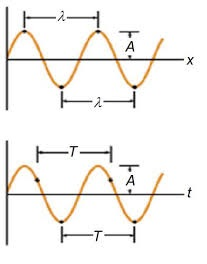
\includegraphics[scale=1]{hull_hossz.jpg}
\caption{Az ábrán láthatjuk egy szinuszos hullámnak pontjainak helyzetét egy adott időpillanatban (felső grafikon) és egy adott pontnak az időbeli mozgását (alsó grafikon).}
\end{figure}

A hullámok vizsgálatakor nagyon fontos azok kategorizálása mely sokféle módon történhet. Az első megkülönböztetés az alapján történik hogy hány dimenzióban terjed a zavar és, ennek megfelelően, beszélhetünk: egydimenziós hullámokról (pl. kötélben terjedő zavar), síkhullámokról (vízen, vagy akármilyen sík felületen kialakuló, hullámok) és térbeli hullámokról (a háromdimenziós térben terjedő hullámok mint például a hang). A következő kategorizálás a terjedési irány és rezgési irány helyzetén alapszik, ha párhuzamosak akkor longitudinális, ha merőlegesek akkor pedig tranzvezális hullámról beszélünk. Végül a hullámfront (azonos fázisú pontok által rajzolt vonal, sík) alakja is megkülönbözteti a hullámokat (pl. sík, henger, gömb, vonal...). 

% ----------------------------------------------------------------
\subsection{Állóhullámok}

Nézzük most a hullámok terjedésének azt a speciális esetét amikor egy megfeszített húrt megpendítünk. Ekkor a húr két vége rögzítve van és ezért a keletkezett hullám és a visszaverődő hullám interferál, ilyenkor a két hullámfüggvény egyszerűen összeadódik és ezért az
$$\Psi(t,x)=\Psi_{\rightarrow} (t,x) + \Psi_{\leftarrow} (t,x)=A'\cdot sin(\omega t-kx + \varphi)- A''\cdot sin(\omega t+kx + \varphi ')$$
általános képletet kapjuk, amit továbbírhatunk a következő alakba felhasználva hogy $A'=A''$ és egy trigonometrikus azonosságot
$$ \Psi = A \sin(k x + \beta) cos(\omega t + \alpha) $$
Ebből a képletből lehet leginkább látni hogy az idő és a hely függés két külön tagban szerepel aminek eredménye az lesz hogy a hullám látszólag állni fog tehát pontyai mindig azonos amplitúdóval rezegnek. A végső megoldás keresésének érdekében feltételezzük hogy a húr a két végén rögzítve van, $L$ hosszú, az x tengellyel párhuzamos és az origó az egyik vége akkor $\Psi(0)=\Psi(L)=0$, ezeket a megoldásokat beírva a függvénybe azt kapjuk eredményül hogy $\alpha=0$ illetve azt hogy ilyen hullámok csak adott diszkrét hullámszámoknál jöhetnek létre:

$$ k = n\dfrac{\pi}{L}; \quad n = \text{1, 2, 3, ...} $$
$$\lambda=\dfrac{2\pi}{k}=\dfrac{2L}{n}$$
$$\omega=kc=\dfrac{n\pi c}{L}$$
Az állóhullámoknak két különleges pontja a térben a duzzadóhely és a csomópont, ezeket is legegyszerűbben a húrmodellel lehet szemléltetni: a duzzadóhely az a pontja a közegnek amely a maximális amplitúdóval rezeg (a két hullám maximálisan erősíti egymást), a csomópont pedig az amely pedig áll (a két hullám kioltja egymást). Fent láttuk hogy a lehetséges diszkrét frekvenciák mindig egymásnak az egész számú többszörösei és ezeknek speciális elnevezésük is van, az \textit{n}=1-et hívjuk alapfrekvenciának és minden $n>1$-re n-edik felharmonikusról beszélünk.
\begin{figure}[h!]
    \centering
    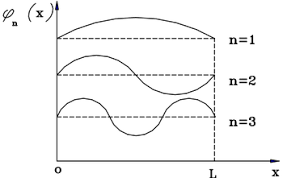
\includegraphics[scale=.5]{allohullam.png}
    \caption{Állóhullámok vázlata.\cite{mintamuszer}}
\end{figure}

%-----------------------------------------------------------------
\subsection{Hanghullámok}
A hang az egyik leggyakoribb hullám a természetben hiszen az élőlények nagy része ezzel kommunikál. Ennek a hullámnak fizikai tulajdonságait vizsgálva azt mondhatjuk hogy egy longitudinális mechanikai gömbhullámról van szó, ez azt jelenti hogy ha egy pontszerű forrásból indül a regés akkor gömb alakú hullámfrontok keletkeznek és a deformáció iránya azonos a terjedési iránnyal. A hang, ezen kívül, mint minden mechanikai hullám csak közegben tud terjedni (pl. levegő). Hanghullámok keltése bármilyen olyan rezgéssel lehetséges mely zavart visz a közegbe, feltéve hogy frekvenciája a hallható tartományon belül van (20-20000 Hz). Sokszor szokás a hangokat felerősíteni, főleg hangszereknél, úgynevezett rezonátorokkal, ezek általában fa dobozok szoktak lenni melyekben a hang úgy verődik vissza a falakról hogy növeli amplitúdóját (hangosabb lesz).

% ----------------------------------------------------------------
\subsection{Fourier transzformáció}

A Fourier transzformáció egy matematikai művelet mely egy $F(t)$ függvényből generál egy $f(\omega)$ függvényt. A fizikában általában $F(t)$ egy időtől, míg $f(\omega)$ egy körfrekvenciától függő függvén, ezért szokták a $F(t)$ Fourier transzformáltját frekvencia spektrumnak is nevezni. Ennek a műveletnek az alapjait a Fourier sorfejtés elvében találjuk mely szerint bármilyen periodikus jelet harmonikus jelek összegére lehet felbontani, tehát egyszerűbben bármilyen periodikus jelet felírhatunk mint szinuszok és koszinuszok összege. Ennek egy általánosítása a Fourier transzformáció mely bármilyen jelre alkalmazható, képlete:
\begin{equation}
f(\omega) = \dfrac{1}{\sqrt{2\pi}} \int^{\infty}_{-\infty} F(t) \cdot e^{i \omega t} \D t
\end{equation}
Labview programunkban viszont nem pontosan ezt használtuk hanem az úgynevezett FFT (Fast Fourier Transform) melynek előnye az hogy lehet őt alkalmazni diszkrét pontokra is, mint amiket a mérőkártya rögzít a mérés során. Ennek a transzformációnak a menete sokkal bonyolultabb mint az előző, ezért inkább nem részletezzük. Összegzés képen ezekről a műveletekről annyit kell tudnunk hogy nagyon hasznosak a fizika minden területén és fő céljuk az hogy egy időben változó jelnek elkészítsék a frekvenciafelbontását. Vegyünk például egy tisztán szinuszos jelet amit egy adott $f$ frekvenciával változik, ha ennek a jelnek vesszük a Fourier transzformáltját egy olyan függvényt kapunk mely mindenhol nulla kivéve az $f$ frekvencia helyen.

\begin{figure}[!h]
\centering
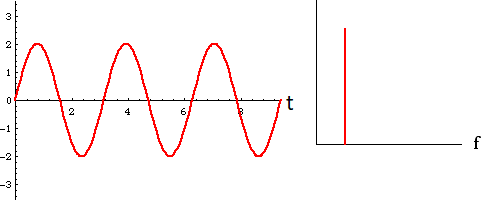
\includegraphics[scale=1]{PowerSpectrum1.png}
\caption{$2 \sin(\omega t)$ (bal), Fourier transzformált (jobb)}
\end{figure} 
Az általunk végzett kíséletben hanghullámokat vizsgálunk melyek sose követnek tiszta harmonikus rezgést hanem mindig több, különböző frekvenciájú, harmonikus jelek keveréke. Ezek a jelek más más intenzítással jelennek meg és ha minden komponensnek a járulékát szeretnénk látni nincs más hátra mint a Fourier transzformációt alkalmazni hogy felbothassuk a jelet. A transzformált jel frekvencia-amplitúdó grafikonját hívjuk spektrumnak.

% ----------------------------------------------------------------
\subsection{Hullámterjedés megfeszített rugalmas húron}

A \ref{hur_hullam}.\ ábrán egy megfeszített rugalmas húr kicsiny darabjáról látunk egy ábrát. A hullám az $x$-tengely mentén terjed, a húr kitérése $y$ irányú és a húrt $\V{T}(x, t)$ erő feszíti. Ezen kívül felvettük a feszítőerő $x$-tengellyel bezárt $\alpha(x, t)$ szögét.

\begin{figure}[!h]
\centering
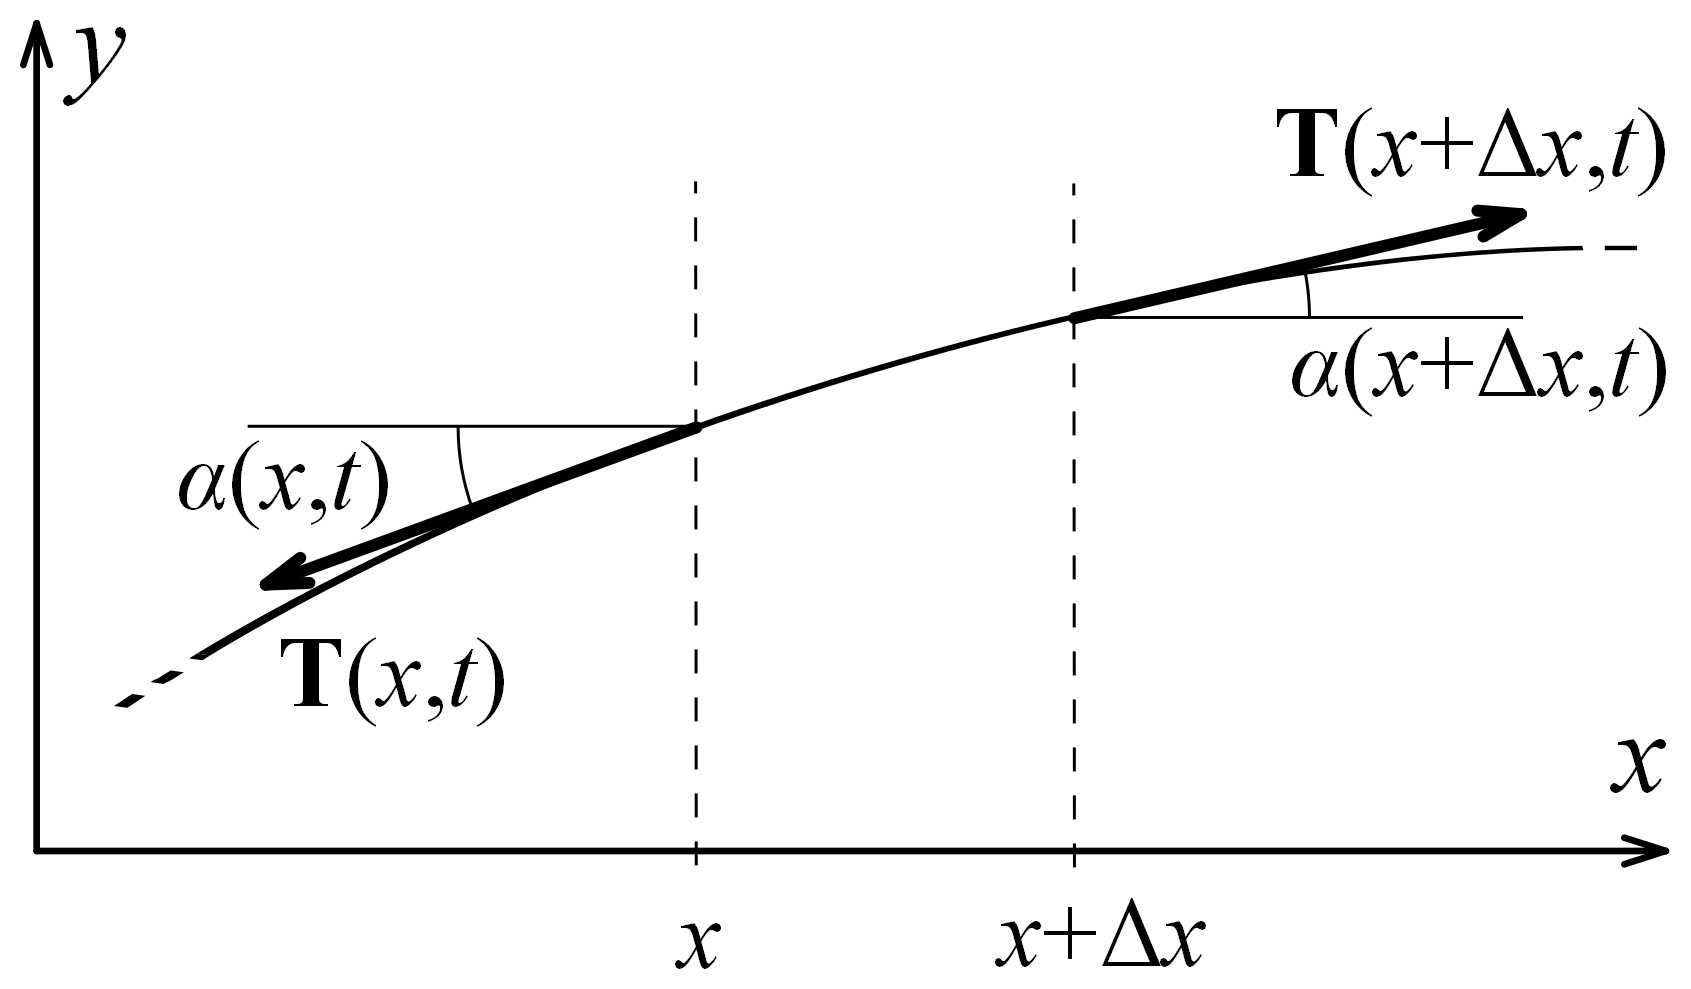
\includegraphics[width = 10cm]{hur_hullam.png}
\caption{Hullám terjedése megfeszített rugalmas húron. \cite{kisfiz1}}
\label{hur_hullam}
\end{figure}

A húrdarabra felírthatjuk a mozgásegyenletet,
$$ \Delta F_y = \Delta m a_y, $$
ahol az $y$ irányú erő
$$ \Delta F_y = T_y(x + \Delta x, t) - T_y(x, t) = $$
$$ = T(x + \Delta x, t) \cdot \sin\alpha(x + \Delta x, t) - T(x, t) \cdot \sin\alpha(x, t). $$
Felhasználva, hogy $T(x, t) \approx T = \text{állandó}$ és $\alpha(x, t) \ll 1$
$$ \Delta F_y = T \left[ \tg\alpha(x + \Delta x, t) - \tg\alpha(x, t) \right] \approx T \frac{\partial \tg\alpha(x, t)}{\partial x} \Delta x $$
adódik. Továbbá felhasználva, hogy
$$ \tg\alpha(x, t) = \frac{\partial \Psi(x, t)}{\partial x}, \quad a_y = \frac{\partial^2 \Psi(x, t)}{\partial t^2} $$
a mozgásegyenlet felírható
$$ T \frac{\partial^2 \Psi(x, t)}{\partial x^2} = \frac{\Delta m}{\Delta x} \frac{\partial^2 \Psi(x, t)}{\partial t^2} $$
alakban. Ezt összevetve az hullámegyenlet \eqref{hullamegyenlet-1D} képletével a hullám terjedési sebességére
$$ c = \sqrt{\frac{T}{\mu}} $$
adódik, ahol $\mu = \frac{\Delta m}{\Delta x}$ a lineáris tömegsűrűség.



% ================================================================
\section{Spektrumanalizátor program}

A mérésünk nem igényel bonyolult kapcsolásokat vagy számolásokat a lementett adatokkal és ez nagyrészt a hozzá írt Labview és C++ programoknak köszönhető. A program elindításához nyissuk meg a \texttt{spectrum\_analysis.lvproject} fájlt a \emph{LabView NXG 1.0} programmal. Ezután a programban felül a \texttt{Library.sli} fülre menve meg kell adni a projekttel mellékelt, annak mappájában lévő \texttt{frequency\_peaks.dll} fájl helyét.

Ezután a mérés elkezdéséhez nincs más dolgunk mint csatlakoztatni a myDAQ-ot a számítógépünkhöz, az \textit{audio in} bemenetre egy mikrofont kapcsolni, majd a programot elindítva elkezdhetjük a mérést.

A program a myDAQ-hoz csatlakoztatott mikrofonnal egy adott hosszúságú ideig mérést végez. Ezután a mért adatoknak spektrum analízisét hajtja végre. A mérés elindítása után a \ref{labview}.\ ábrához hasonló képet kell látnunk.

\begin{figure}[h]
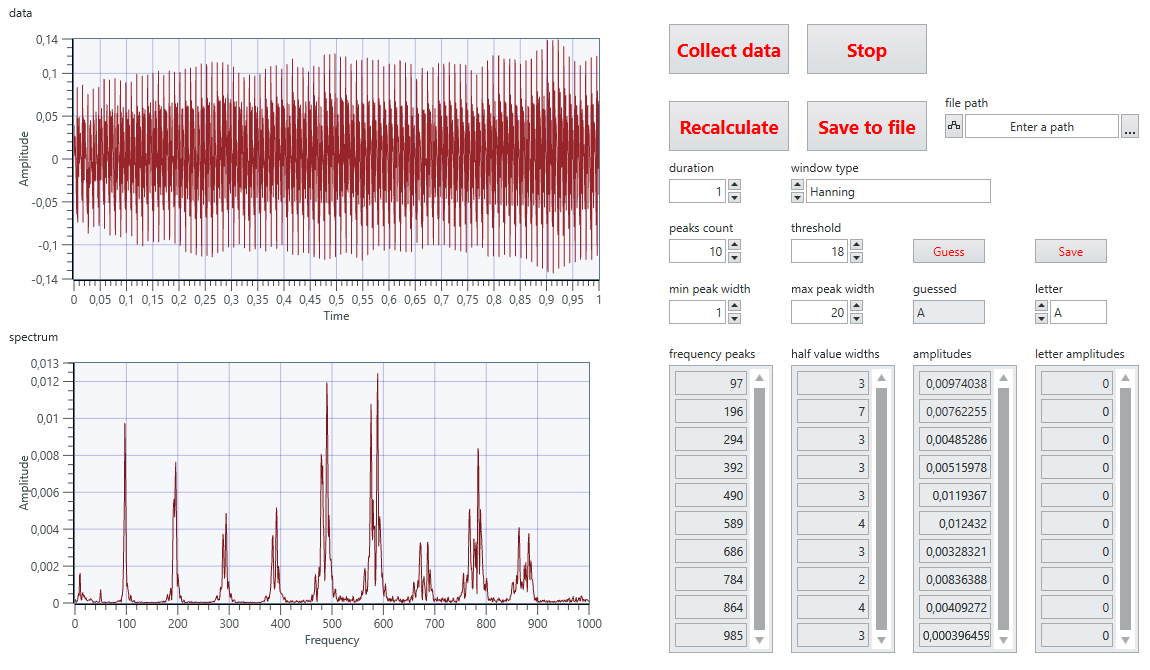
\includegraphics[width=\textwidth]{labview.png}
\caption{}
\label{labview}
\end{figure}

Az ablakban két grafikon van, a felső a mért adatok, az alsó annak a Fourier transzformációja. A programban négy fontos gomb található,
\begin{itemize}
\item \emph{Collect data}, ez indítja el az adatok gyűjtését, annyi másodpercig mér, amennyi a \emph{duration} mezőben meg van adva,
\item \emph{Stop}, ez leállítja a mérést,
\item \emph{Recalculate}, ezzel újra lehet ugyanarra az adatokra számítani a Fourier transzformációt és a csúcsokat. Ez a gomb akkor hasznos, ha a program nem találja meg egyből a csúcsokat a beállított paraméterekkel, vagy rossz ablakot állítottunk be a Fourier transzformációhoz,
\item \emph{Save to file}, ez elmenti a talált csúcsokat a \emph{file path} mezőben megadott fájlba. Ezt szöveges formátumban teszi meg és a fájl végére írja az adatokat, így a korábban mentett adatokat nem írja felül.
\end{itemize}
Még kívül 7 paramétert állíthatunk,
\begin{itemize}
\item \emph{duration} a mérés időtartama másodperben,
\item \emph{peaks count} a keresett csúcsok száma,
\item \emph{threshold} a keresett csúcsok minimális magassága dB-ben,
\item \emph{min peak width}, \emph{max peak widht} a keresett csúcsok minimális és maximális szélessége Hz-ben,
\item \emph{file path} az a fájl, ahova a \emph{Save to file} gomb elmenti az adatokat,
\item \emph{window tipe} a Fourier transzformációhoz használt ablakfüggvény. Alapvetően a \emph{Flat top} és \emph{Hanning} ablakokat használjuk, ezek rendre a pontos amplitúdó és a pontos frekvencia méréséhez használhatóak.
\end{itemize}

A program által talált frekvenciacsúcsok adatait a \emph{frequency peaks}, a \emph{half value widths} és az \emph{amplitudes} táblázatokból tudjuk leolvasni. Ezek rendre a frekvenciacsúcsok helyei Hz-ben, a frekvenciacsúcsok félértékszélessége Hz-ben és a frekvenciacsúcsok amplitúdói V-ban.

A \emph{magánhangzók spektrumának vizsgálata} méréshez ezen kívül még használjuk a \emph{Save} gombot, ami a \emph{letter} mezőben megadott betűhöz rendeli a legutóbbi mérésből származó frekvenciacsúcsok értékeit. Ha az összes magánhangzóhoz elmentettük a frekvenciacsúcsok nagyságát, akkor egy új felvételt készíthetünk, és ezután a \emph{Guess} gombra kattintva a program megpróbálja kitalálni, hogy milyen magánhangzót mondtunk ki ebben a mérésben, amit az alatta lévő \emph{guessed} ablakban láthatunk.



% ================================================================
\section{Magánhangzók spektrumának vizsgálata}
Az emberi kommunikációnak a legalapvetőbb formája a beszéd ami sok évezredeken át fejlődött az és változott az emberek igényei és kultúrájuk szerint. Az embereknek ezen képessége nemcsak a hangszálaknak köszönhető hanem kiemelkedő agyi képességeiknek is. Egy adott szó kiejtése egy összetett folyamat melynek során a tüdőnkből kiáramló levegőnek hatására a hangszálaink rezegni kezdenek hangot produkálva amelyet majd a szájüregünk és nyelvünk segítségével modulálunk, az így generált hangot az agyunk egy adott tárgyhoz vagy fogalomhoz társítja.\\ 
Kísérletünkben csakis a magánhangzók spektrumát vizsgáljuk mivel ezek olyan speciális hangok melyeket úgy keltünk hogy szájüregünket rezonátornak használjuk és ezért több másodpercig is tudjuk őket "énekelni". Ezzel szemben a mássalhangzókat ajkunk és nyelvünk mozgatásával kéltjük és nem lehet őket folytonosan énekelni ezért spektrumuk vizsgálata nagyon nehéz. Visszatérve a magánhangzókra azt mondtuk hogy a szánk rezonátorként működik a kiejtésüknél, de pontosan mit is jelent ez? Nos biztosan mindenki próbálta már azt csinálni hogy egy levegővel teli lufinak a száját megfeszítve hangot hallunk amikor a levegő kiáramlik a lufiból és minél feszesebben tartjuk a száját annál magasabb lesz a hang, testünk hasonlóan működik csak a lufi szerepét a tüdőnk a "száj" szerepét pedig a hangszálak játsszák. Aztán az így kialakult hang a torkunkon és szánkon keresztül terjed ahol folyton visszaverődik ezeknek falairól és így egy vételen sok hanghullám szuperpozícióját halljuk. Minden egyes kombináció más más végeredményt produkál és ezek közül van 9 speciális eset amit magánhangzónak hívunk. 

% ----------------------------------------------------------------
\subsection{Mérés menete}
Mérésünk során ezen 9 speciális hangnak (a, á, e, é, o, ő, u, ű) a Fourier spektrumát vizsgáltuk három különböző emberre, annak reményében hogy hasonlóságokat tapasztalunk a hangokban. Az adatgyűjtést a myDAQ mérőkártyával és egy hozzá írt Labview programmal végeztük, a mérés menete nem túl bonyolult elég a mérőkártyához egy mikrofont kapcsolni és a program elindítása után a magánhangzókat kiejteni, minden hangot legalább háromszor ajánlatos mérni. Kiemelten fontos az hogy hangosan ejtsük ki a hangokat és ha laptopról mérünk az ne legyen töltőn, ennek oka az hogy a mérőkártya a hangerősség mérést feszültségmérésre vezeti vissza és ebben jelen van egy nagyon gyenge 50 Hz-es zaj ami felerősödik a töltés során ( valószínűleg a hálózat miatt). Ez agában nem okoz kárt a mérésben hiszen a program a csúcs keresést az FFT-ben alapból úgy csinálja hogy kizárja ezt a zaj, viszont ennek felharmonikusait, főleg az elsőt, nem lehet kizárni a spektrumból mivel a hangunk frekvenciatartományában van és ezért az egyetlen módszer a helyes méréshez az ha sokkal nagyobb amplitúdójú a hangunk frekvenciája mint a zajé.\\
Miután végeztünk a méréssel az adatokat egy text file-ban találhatjuk melyet bármilyen adatkezelő programmal vizsgálhatunk. Mivel ebben az esetben nem kell nehéz műveleteket végezni az adatokkal, bőven megfelel az Excel mint program. Miután átmásoltuk az adatokat grafikonon ábrázoljuk az azonos hangokhoz tartozó frekvencia amplitúdókat, ennél a lépésnél nem fontos hogy minden frekvencia érték jelen legyen a grafikonon hiszen ami minket érdekel a különböző felharmonikusok egymáshoz képesti erőssége. 
\begin{figure}[h]
\centering
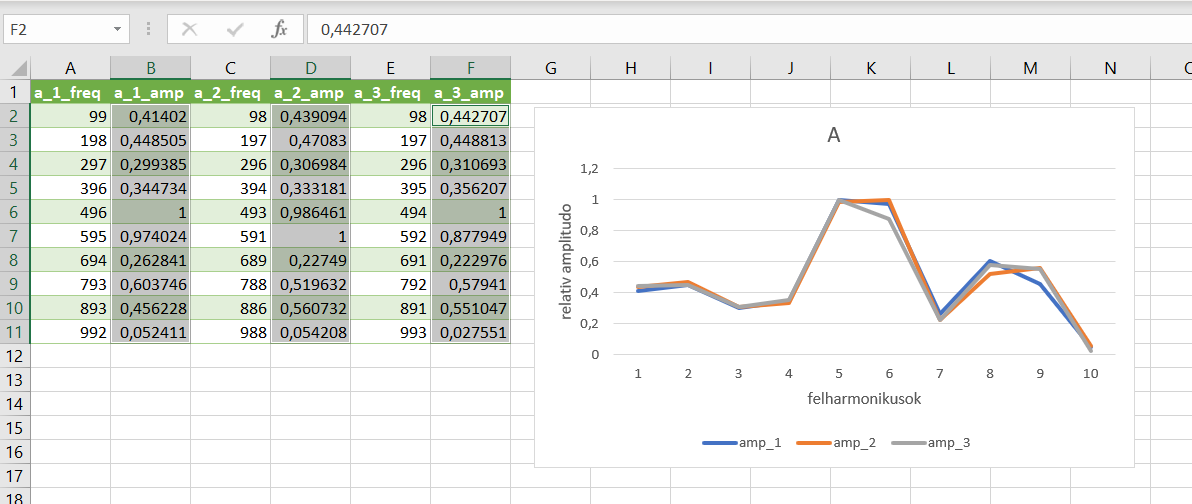
\includegraphics[width=\textwidth]{minta.png}
\caption{Kijelölt rész az ábrázolandó.}
\label{1ábra}
\end{figure} 
Az így kapott ábrákról könnyen leolvasható a felharmonikusok aránya a magánhangzók spektrumában.

% ----------------------------------------------------------------
\subsection{Következtetések} 
A kapott táblázatokból látható hogy a spektrumban a megjelenő frekvenciák tényleg az első (alapfrekvencia) egész számú többszörösei(lásd \ref{1ábra}), hibahatáron belül. Ha összegyűjtjük minden hang alapfrekvenciáját egy táblázatba, meglepő módon azt tapasztaljuk hogy ezek nagyon közel állnak egymáshoz ha egy alanynak a hangjait vizsgáljuk  viszont eltérnek az alanyok között. 
\begin{table}[h]
\centering
\begin{tabular}{c|c|c|c}
 & Csanád (Hz) & Zeno (Hz) & Lukács (Hz) \\ 
\hline 
A & 98 & 108 & 137 \\ 
Á & 101 & 114 & 133 \\ 
E & 106 & 110 & 147 \\ 
É & 107 & 113 & 146 \\ 
I & 113 & 152 & 148 \\ 
O & 114 & 119 & 182 \\ 
Ő & 114 & 123 & 197 \\ 
U & 126 & 110 & 183 \\ 
Ű & 128 & 155 & 159 \\ 

\end{tabular} 
\caption{Alapfrekvenciák átlagértékei minden betűre}
\label{1tábla}
\end{table}  
A táblázatról (\ref{1tábla}) jól látható hogy hármunk közül Csanádnak van a legmélyebb hangja míg Lukácsnak a legmagasabb. Látva ezt az eredményt, viszont, felmerül a kérdés hogy mégis hogyan lehetnek ennyire másak a hangok ha alapfrekvenciájuk csupán 30-50 Hz változik? És mégis hogyan lehetséges az hogy ha mindenki képes kiejteni ugyan azt a magánhangzót akkor is ha más más alapfrekvencián beszél?\\
Ezekre a kérdésekre a választ úgy kapjuk meg ha ábrázoljuk a felharmonikusok amplitúdóit egy grafikonon. Ezen diagramok vizsgálatából kiderül hogy, hiába minden ember más más alapfrekvenciával ejti ki a hangokat, azért tudunk kommunikálni mert úgy tudjuk átalakítani szánk és ajkunk alakját hogy a visszaverődő hullámok adott felharmonikusai egy adott sémát kövessenek amely az adott hangot jellemzi. Vegyük például az "Ő" hangnak mindhárom grafikonját:

\begin{figure}[h!]
\centering
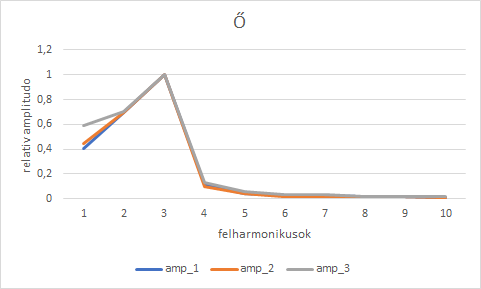
\includegraphics[scale=0.9]{csanad_o.png}
\caption{Csanád "Ő" betűjének felharmonikusainak aránya.}
\end{figure}
\newpage
\begin{figure}[h!]
\centering
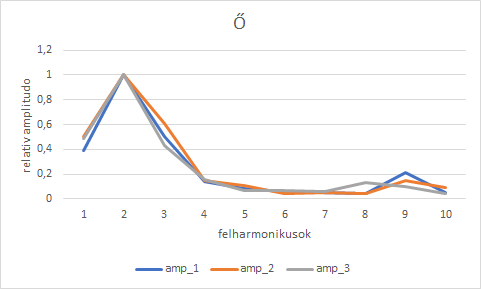
\includegraphics[scale=0.9]{lukacs_o.png}
\caption{Lukács "Ő" betűjének felharmonikusainak aránya.}
\end{figure}
\begin{figure}[h!]
\centering
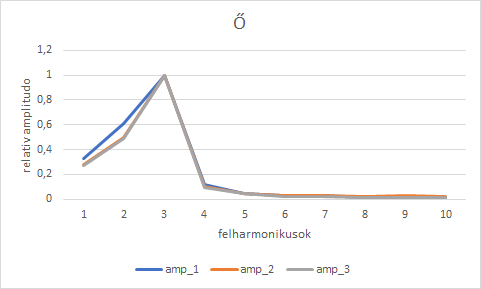
\includegraphics[scale=0.9]{zeno_o.png}
\caption{Zeno "Ő" betűjének felharmonikusainak aránya.}
\end{figure}
Ezekből tisztán látható az hogy az "Ő" betűnek a második és a harmadik felharmonikusa a legerősebb míg a többi gyakorlatilag elhanyagolható hozzájuk képest. Az alábbi diagramokban a különböző betűk felharmonikusainak aránya látható (csak Csanád diagramjait jelenítjük meg).
\begin{figure}[h!]
\centering
\begin{minipage}{.5\textwidth}
  \centering
  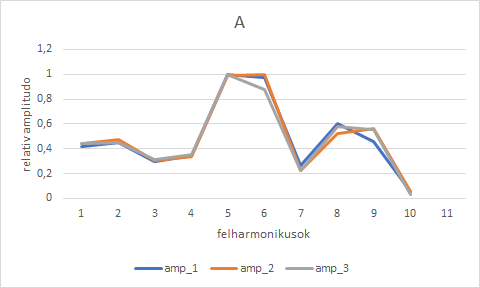
\includegraphics[width=.9\linewidth]{A.png}
\end{minipage}%
\begin{minipage}{.5\textwidth}
  \centering
  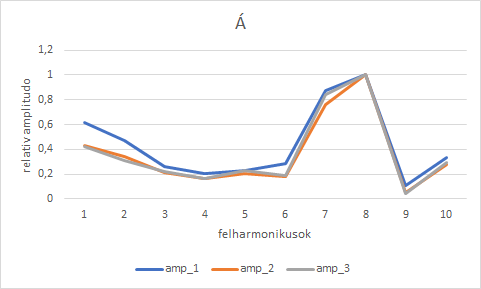
\includegraphics[width=.9\linewidth]{A_1.png}
\end{minipage}
\end{figure}
\begin{figure}[h!]
\centering
\begin{minipage}{.5\textwidth}
  \centering
  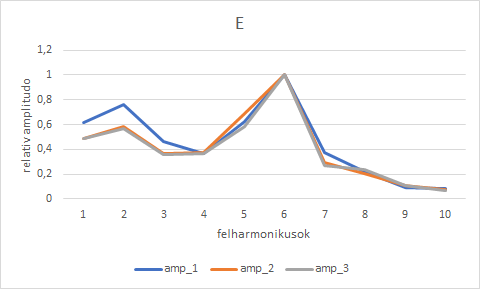
\includegraphics[width=.9\linewidth]{E.png}
\end{minipage}%
\begin{minipage}{.5\textwidth}
  \centering
  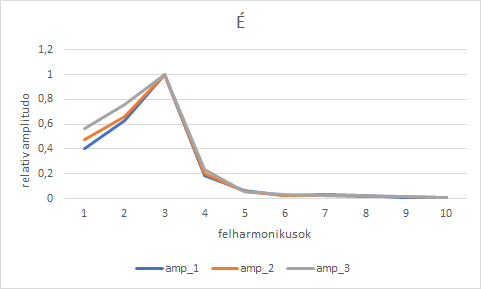
\includegraphics[width=.9\linewidth]{E_1.png}
\end{minipage}
\end{figure}
\begin{figure}[h!]
\centering
\begin{minipage}{.5\textwidth}
  \centering
  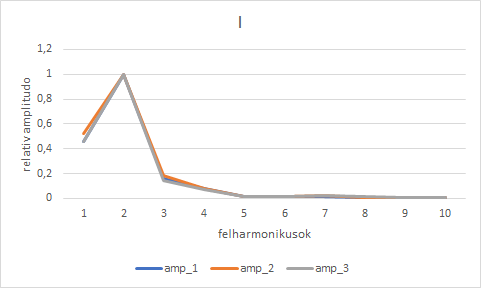
\includegraphics[width=.9\linewidth]{I.png}
\end{minipage}%
\begin{minipage}{.5\textwidth}
  \centering
  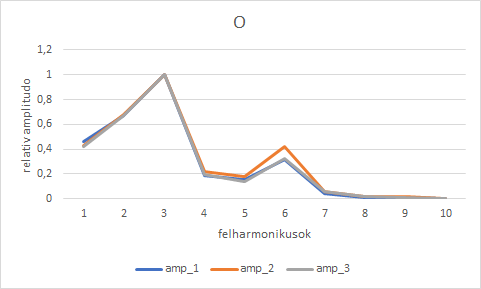
\includegraphics[width=.9\linewidth]{O.png}
\end{minipage}
\end{figure}
\begin{figure}[h!]
\centering
\begin{minipage}{.5\textwidth}
  \centering
  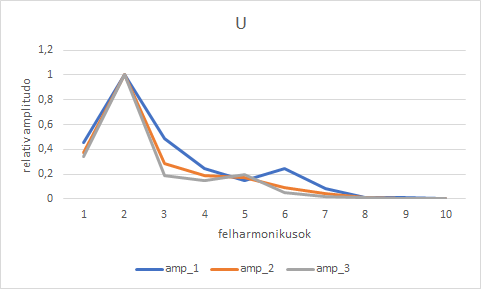
\includegraphics[width=.9\linewidth]{U.png}
\end{minipage}%
\begin{minipage}{.5\textwidth}
  \centering
  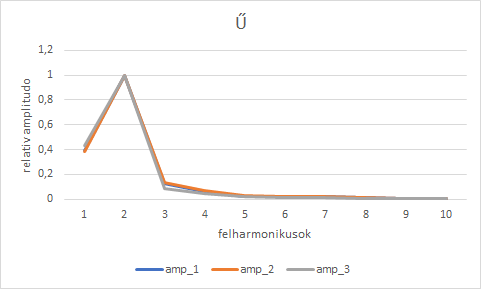
\includegraphics[width=.9\linewidth]{U_1.png}
\end{minipage}
\end{figure}




% ================================================================
\section{Húrok frekvencia spektrumának vizsgálata}

Ebben a mérésben neylon hárfahúrokat feszítettünk meg a \ref{muszer_abra}.\ ábrán látható készülék mintájára és mértük a hangjuk alapfrekvenciáját, amiből meghatároztuk a vastagságukat.

% ----------------------------------------------------------------
\subsection{Elméleti összefoglaló}

Egy mindkét végén rögzített húrban a kialakuló állóhullámok alapfrekvenciáját a
$$ f_0 = \frac{c}{2 L} $$
képlet alapján számolhatjuk, ahol $L$ a rögzítési pontok közti távolság. Korábban láttuk, hogy egy megfeszített húrban a hullámterjedési sebességet meghatározhatjuk a $T$ feszítőerő és $\mu$ lineáris tömegsűrűség ismeretében,
$$ c = \sqrt{\frac{T}{\mu}}. $$
Továbbá a húr anyagának $\rho$ térfogati tömegsűrűsége ismeretében a lineáris tömegsűrűség kifejezhető,
$$ \mu = \rho \frac{d^2}{4} \pi, $$
ahol $d$ a húr átmérője. Ezzel az alapfrekvenciára a
$$ f_0 = \frac{1}{d L \sqrt{\rho \pi}} \sqrt{T} $$
képlet adódik.

Egy húrnál az alapfrekvencia és a feszítőerő mérésével így meghatározható annak vastagsága. Ehhez az $f_0$-$T$ összefüggésre egy $f(T) = C \sqrt{T + T_0}$ alakú függvényt illeszthetünk. $C$ kifejezhető,
$$ C = \frac{1}{d L \sqrt{\rho \pi}}, $$
$T_0$ pedig egy konstans tag, ami magába foglalja a feszítő kar súlyából és a súlyok felfüggesztéséhez használt madzag súlyából származó feszítőerőt.

A méréshez mi neylon hárfahúrokat használtunk, viszont akármilyen más, ismert sűrűségű anyagból készült húr is megfelel a célnak, mint például egy acél húr.

% ----------------------------------------------------------------
\subsection{Mérési elrendezés}

\begin{figure}[h!]
\centering
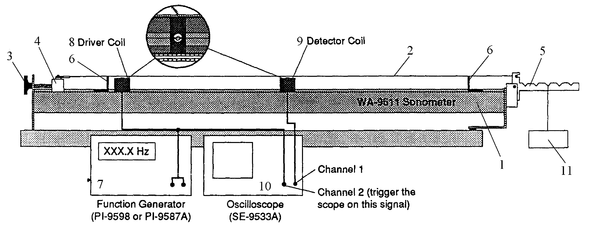
\includegraphics[width =.6\textwidth]{berendezes1.png}
\caption{A mérési berendezés építésének alapjául szolgáló mintakészülék. \cite{mintamuszer}}
\label{muszer_abra}
\end{figure}

\begin{figure}[h!]
\centering
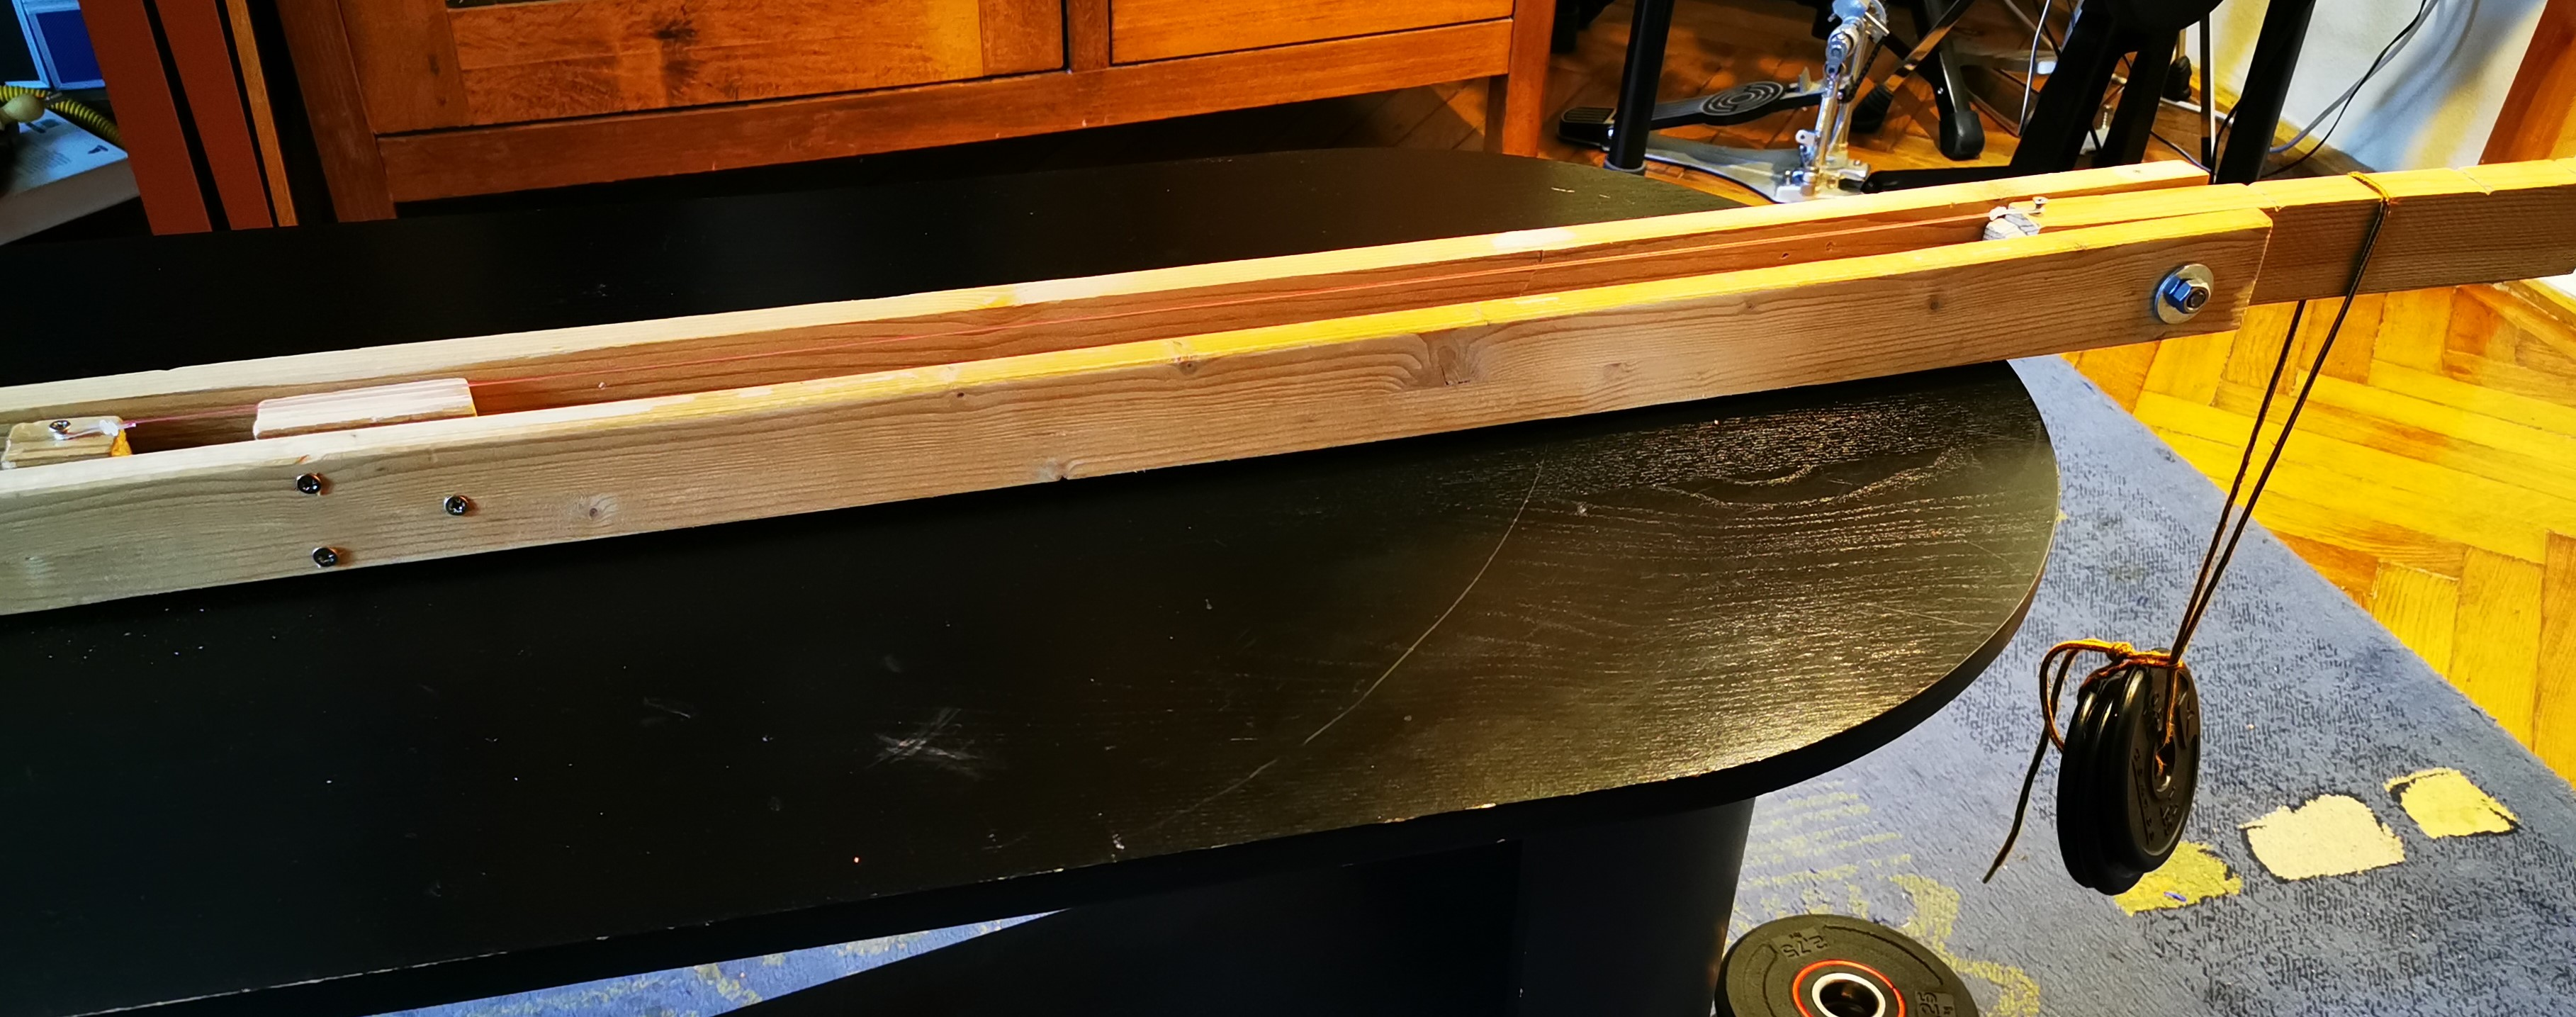
\includegraphics[width = \linewidth]{elejesullyal.jpg}
\caption{A mérőpad.}
\label{muszer}
\end{figure}

A \ref{muszer_abra}.\ ábra mintájára épitettük meg a mérőpadunkat, amit a \ref{muszer}.\ ábrán láthatunk. A pad alapját két párhuzamos farúd alkotja. Az egyik végén a húr egy szabadon forgó rúdra van erősítve, ami nagyjából $20$\,cm-t túl lóg a párhuzamos farudakon. Így ha egy súlyt helyezünk erre az elemre a húrt ismert erővel tudjuk feszíteni. A méréshez ebbe a rúdba $4$ bevágást ejtettünk úgy, hogy a húrt feszítő erő a súlynak rendre $1$, $2$, $3$ és $4$-szerese legyen. Ezt a \ref{erokar}.\ ábrán láthatjuk közelebbről.

\begin{figure}[h!]
\centering
\begin{subfigure}[t]{.4\linewidth}
\centering
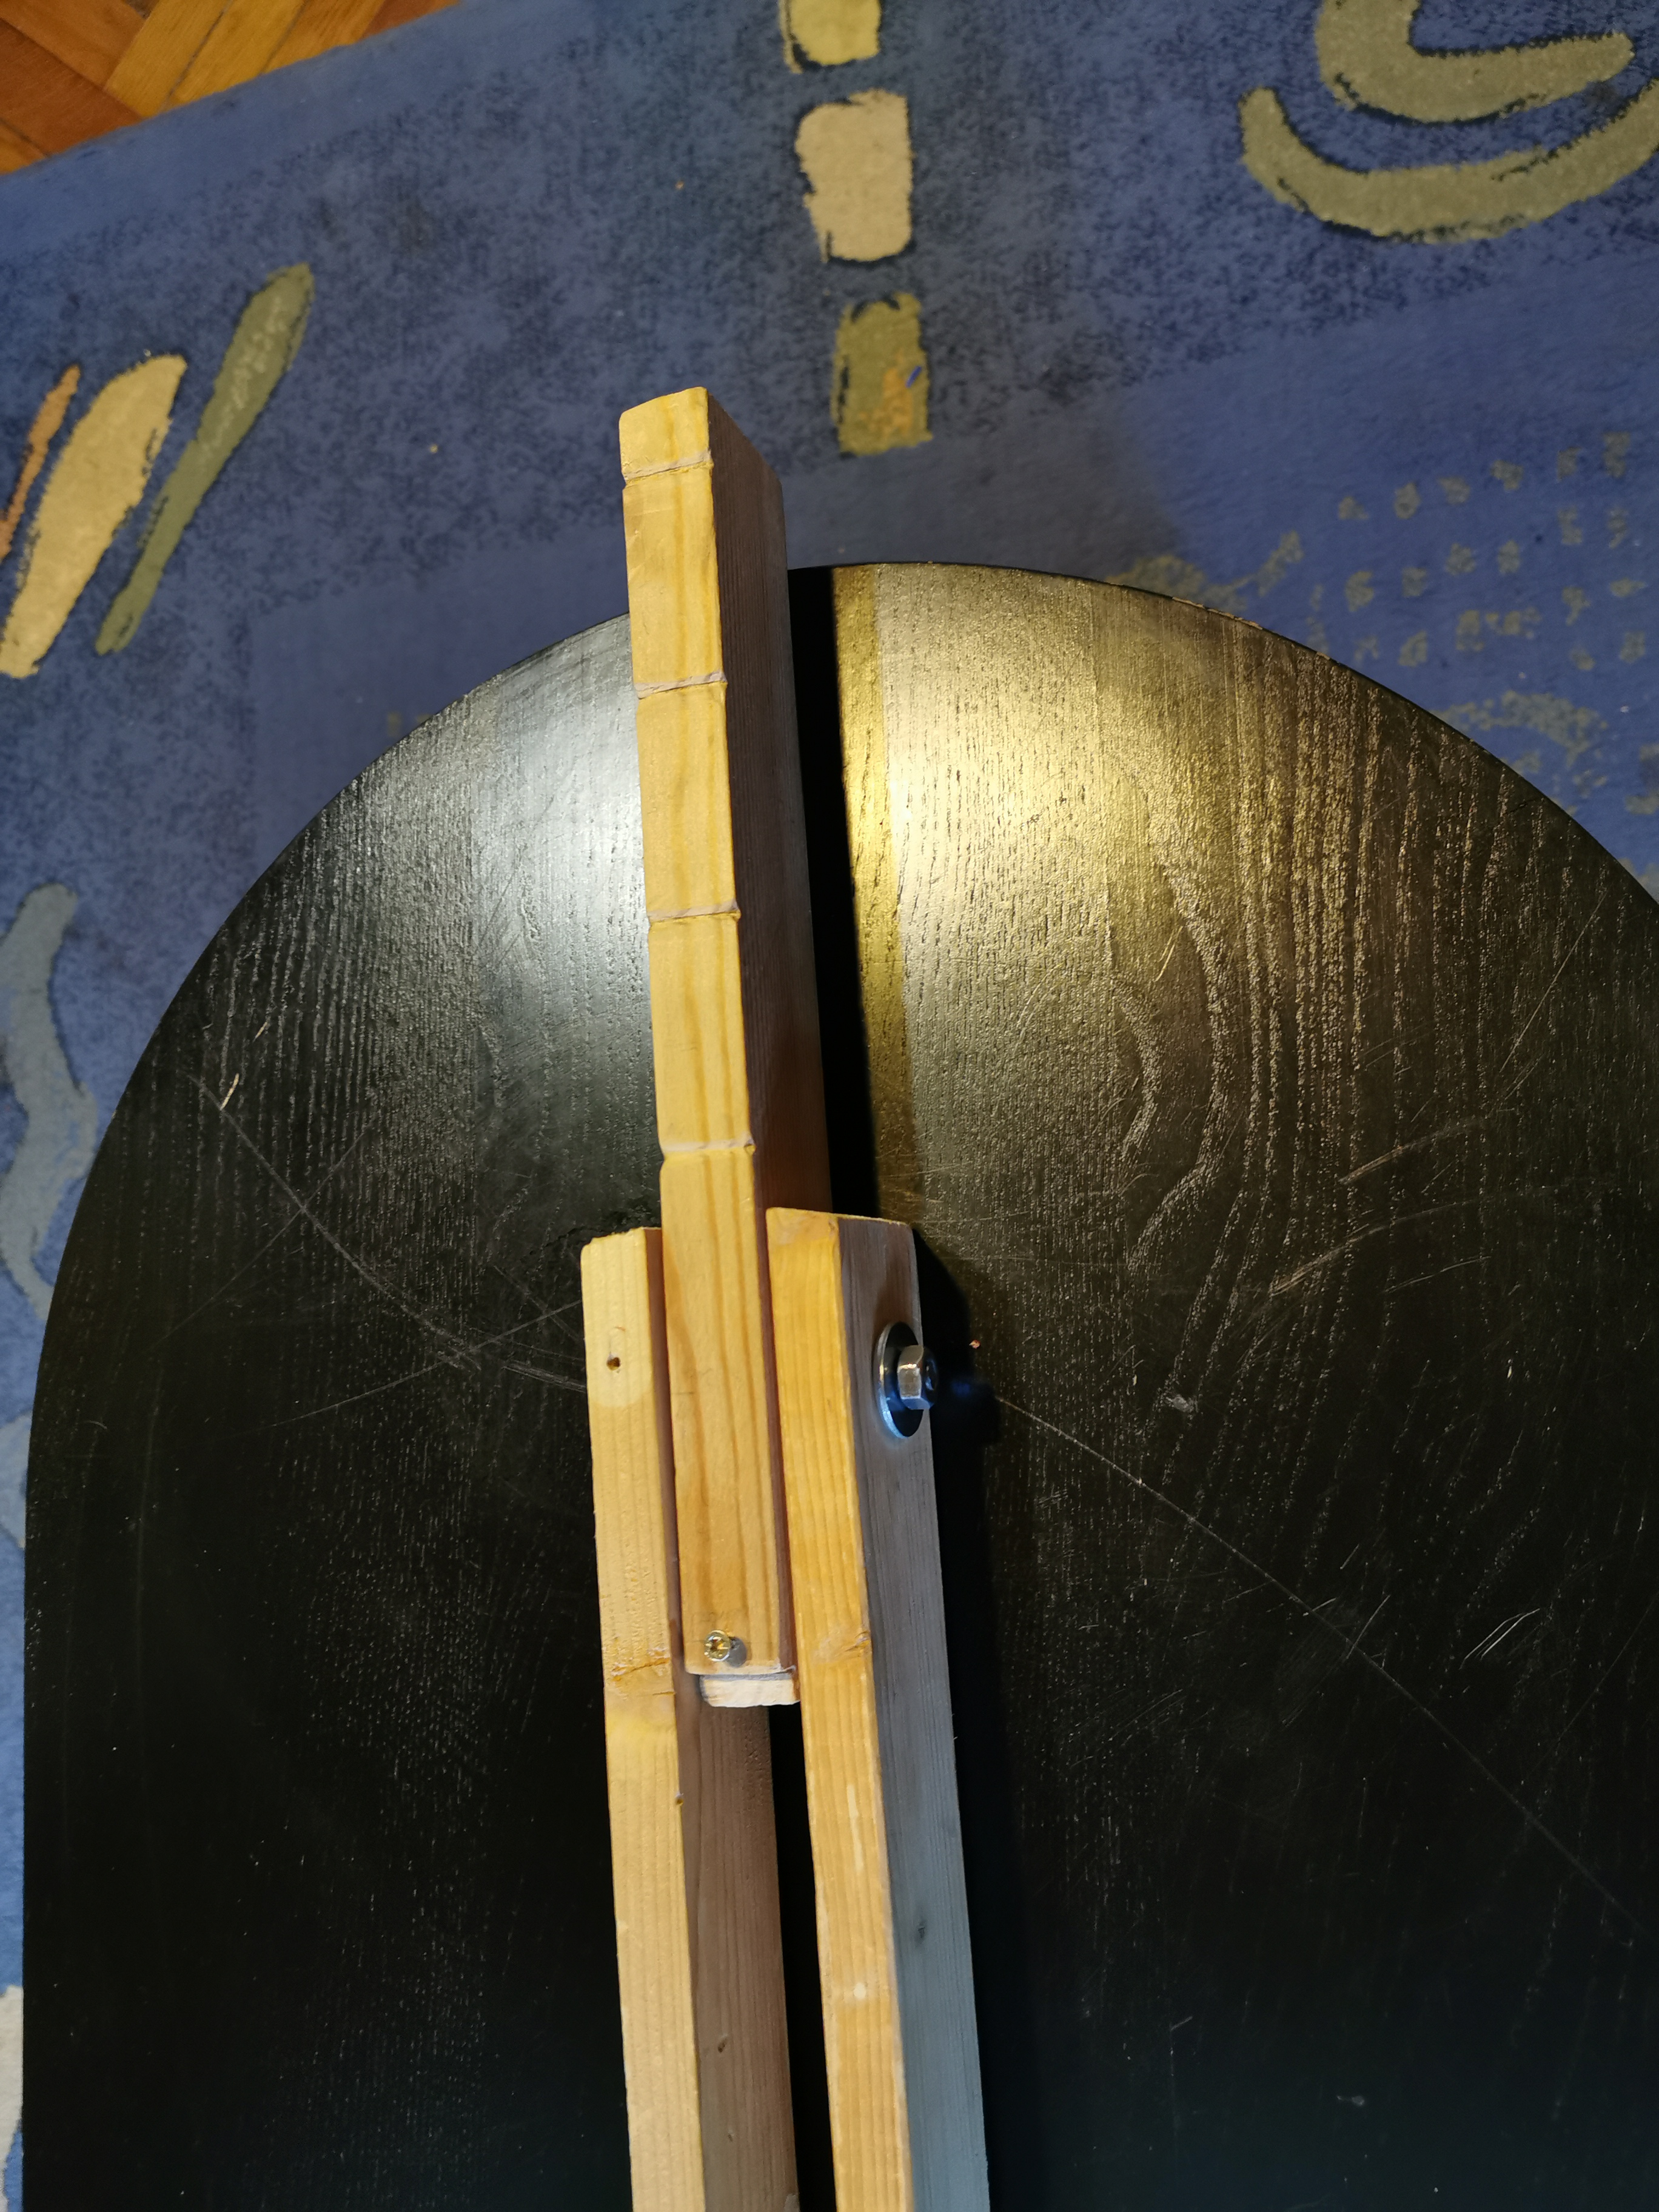
\includegraphics[width=\linewidth]{elejesulynelkul.jpg}
\end{subfigure}%
~~
\begin{subfigure}[t]{.4\linewidth}
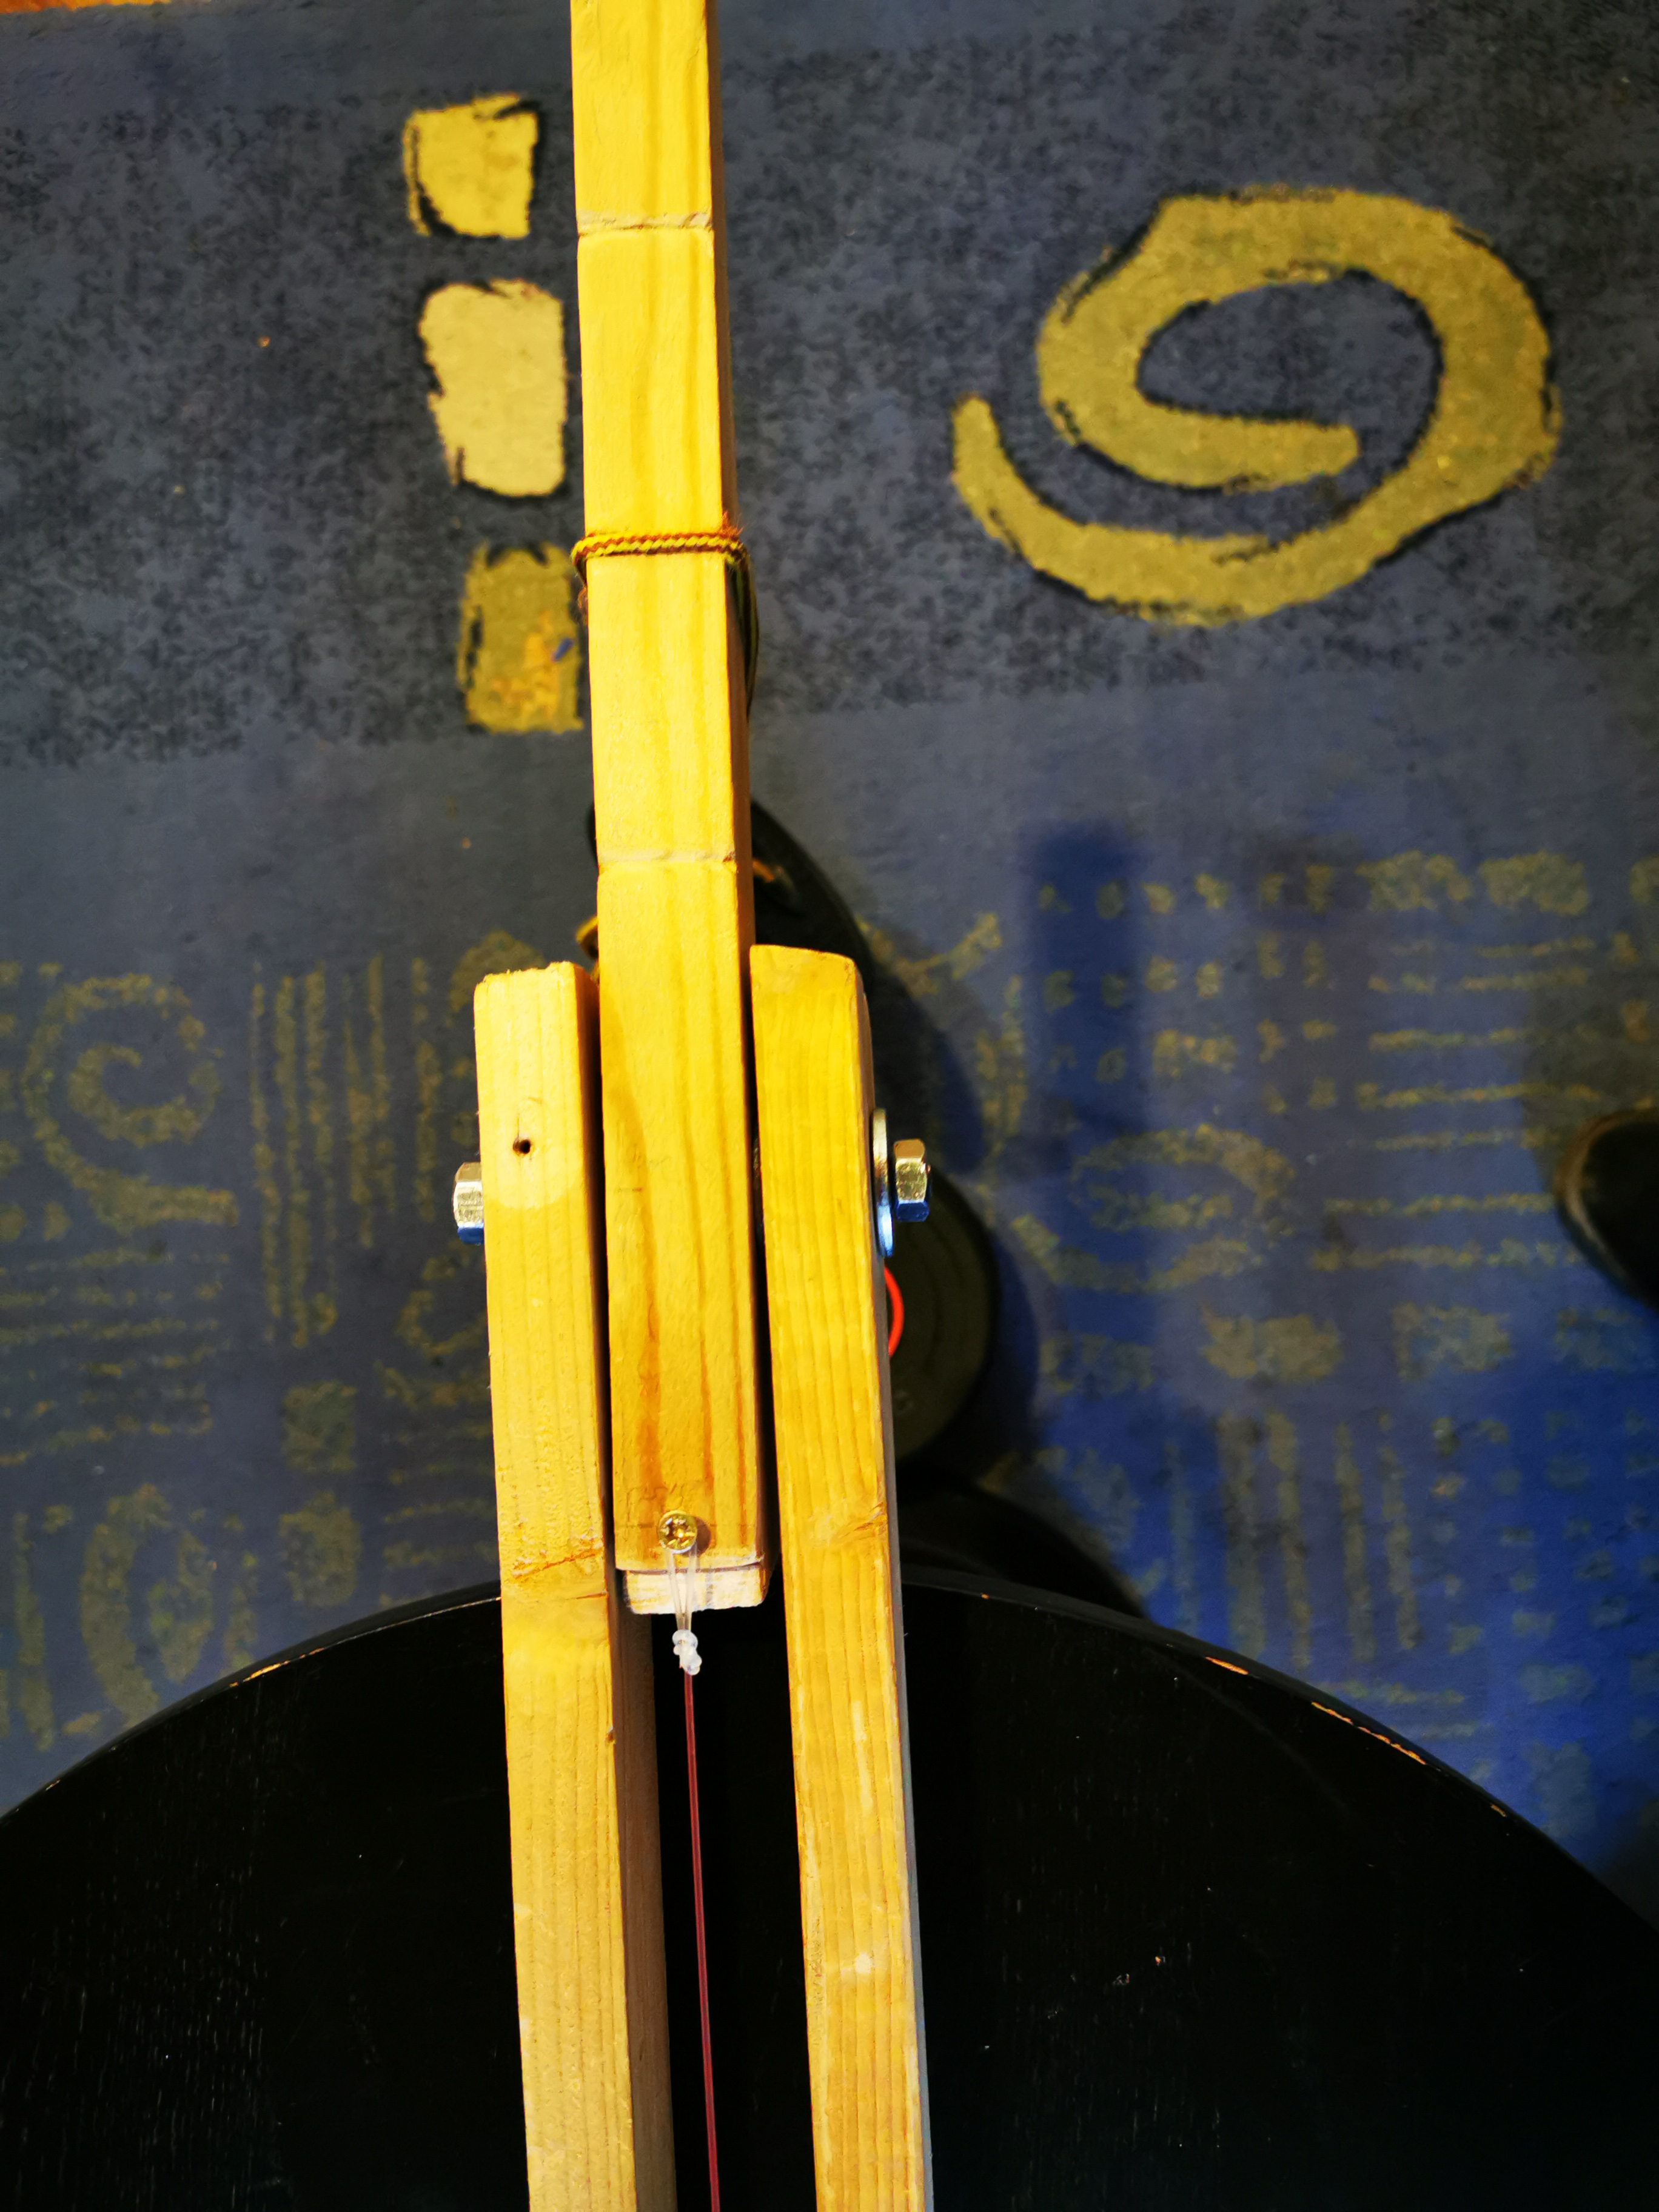
\includegraphics[width=\linewidth]{eleje.jpg}
\end{subfigure}
\caption{A húrt feszítő elem.}
\label{erokar}
\end{figure}

A mérőpad másik végénél két fadarab közé egy menetes szárat erősítettünk. Arra egy másik fadarabot, amin a húr másik vége van rögzítve és egy anyacsavart helyeztünk, így a húr rögzítésének helyét tudjuk mozgatni. Ezt a \ref{menetes}.\ ábrán láthatjuk.

\begin{figure}[h!]
\centering
\begin{subfigure}[t]{.4\linewidth}
\centering
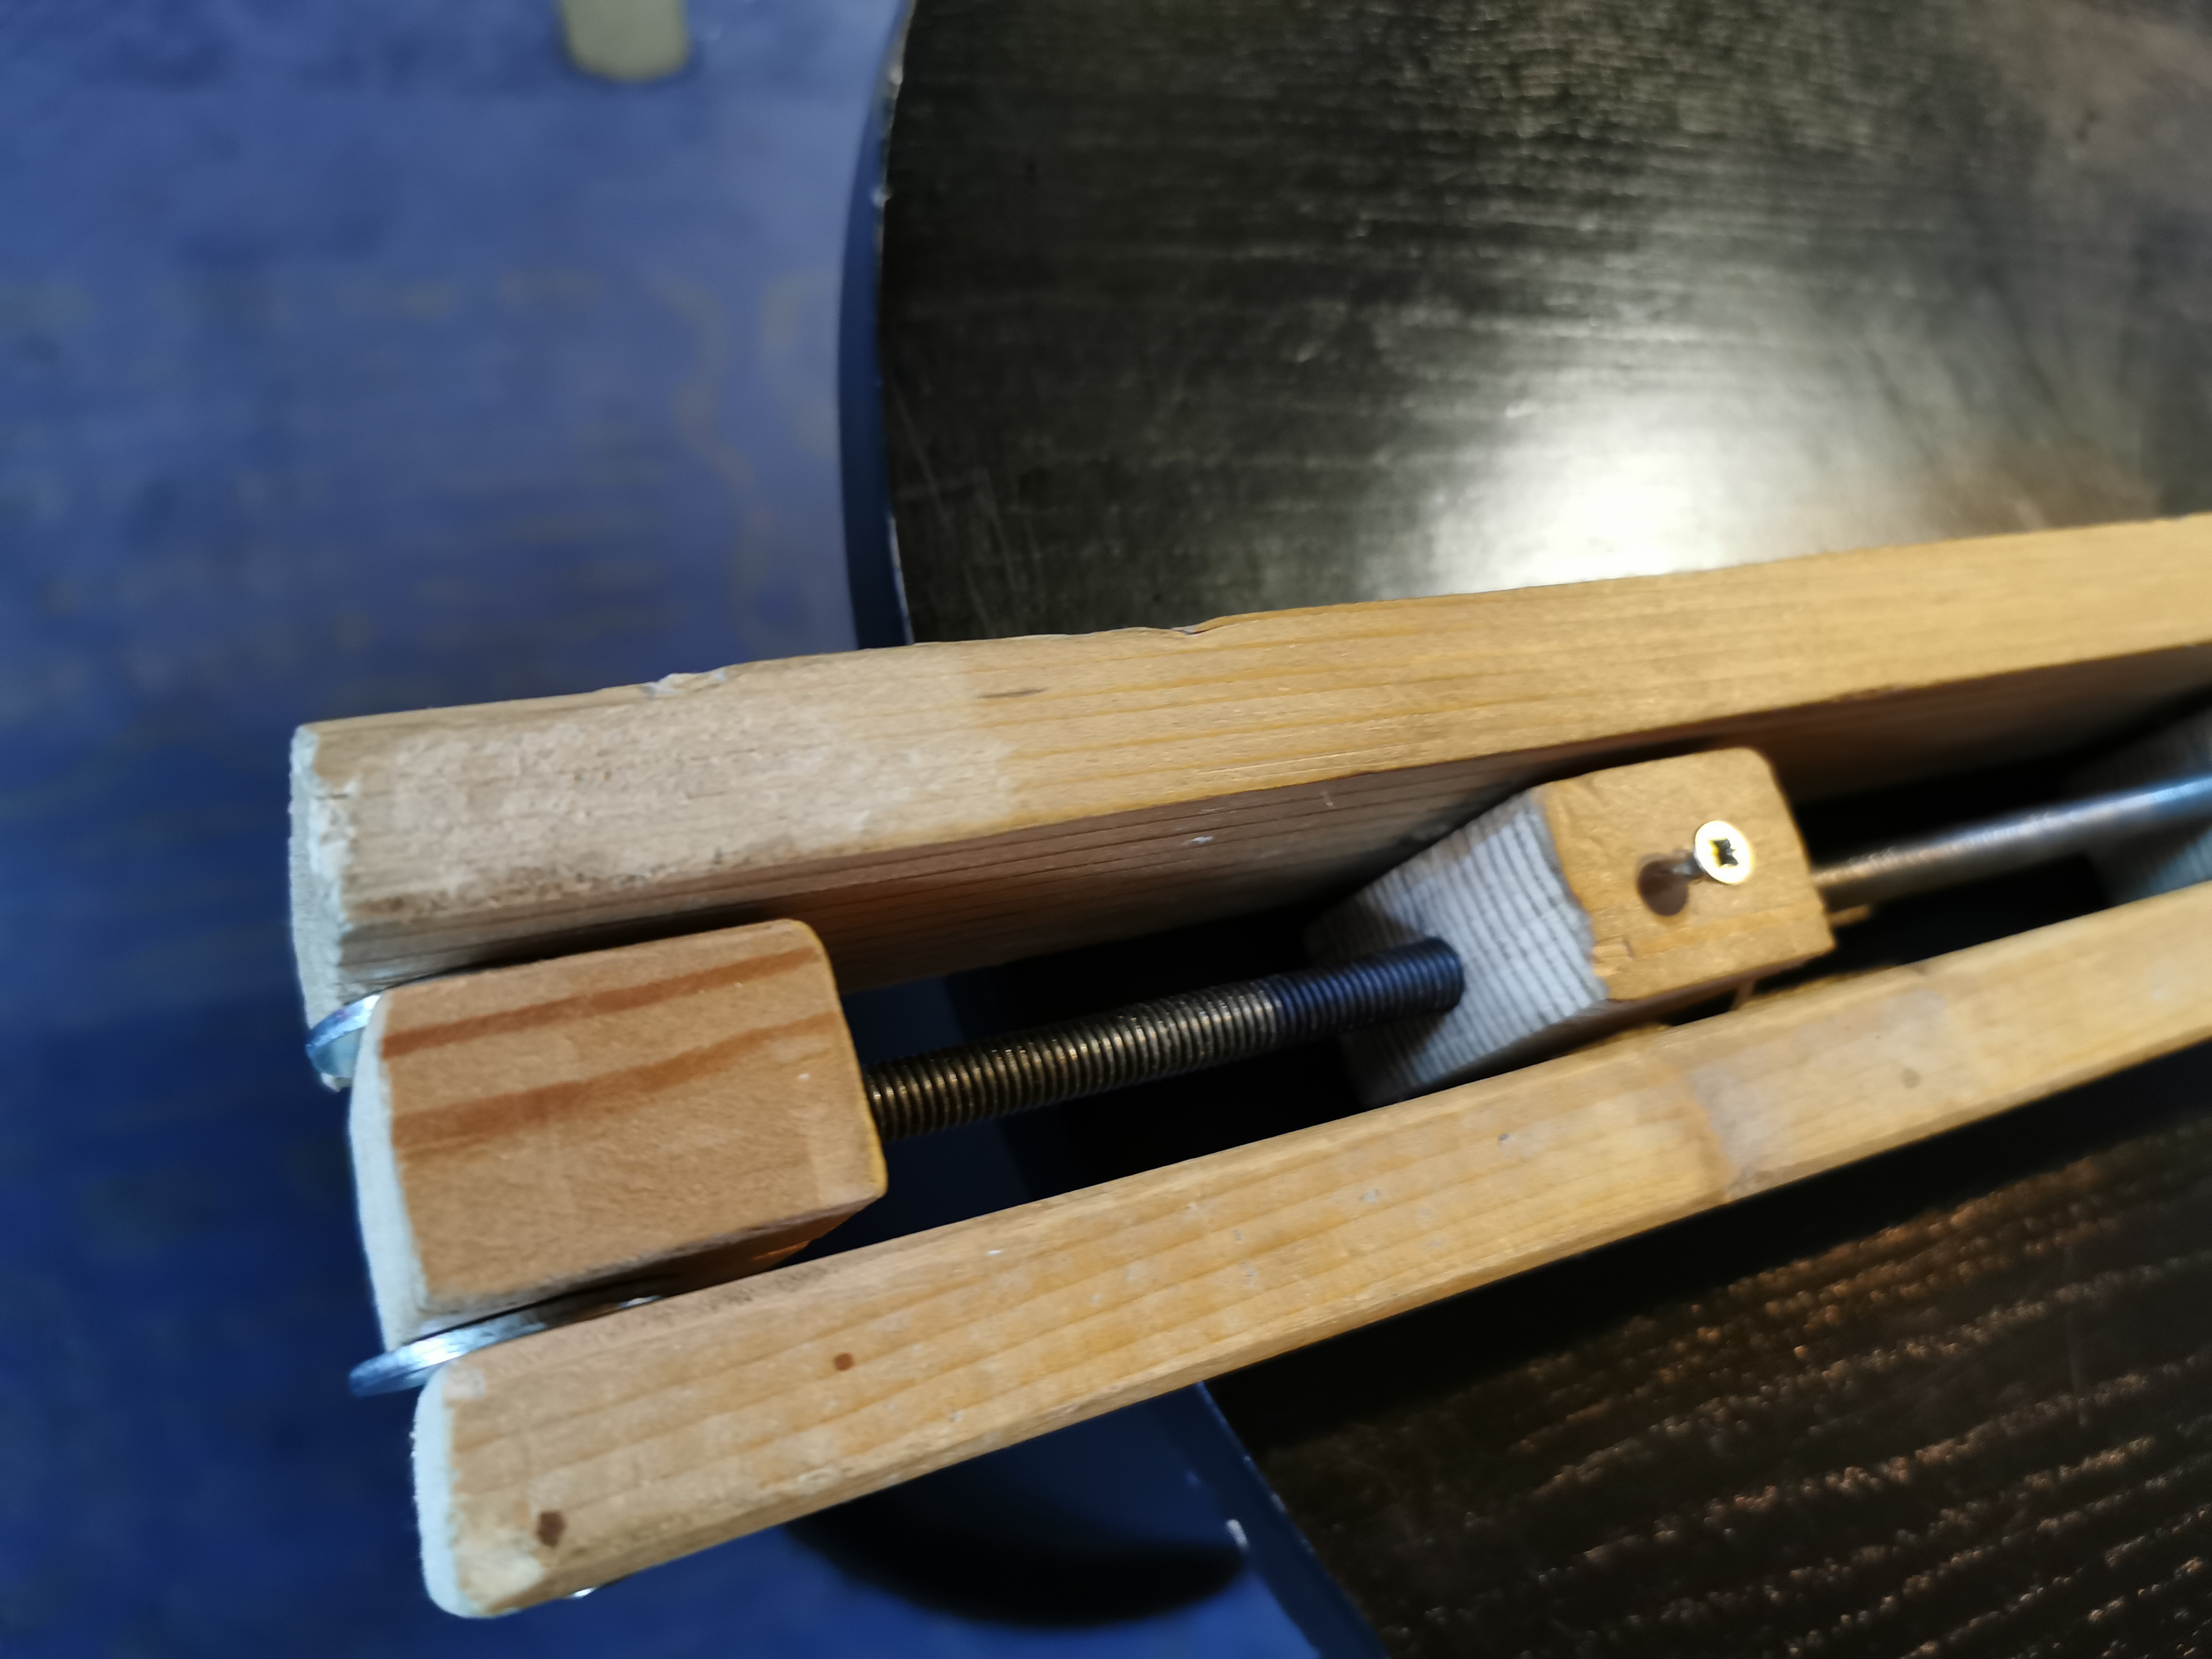
\includegraphics[width=\linewidth]{vegekozel.jpg}
\end{subfigure}%
~~
\begin{subfigure}[t]{.4\linewidth}
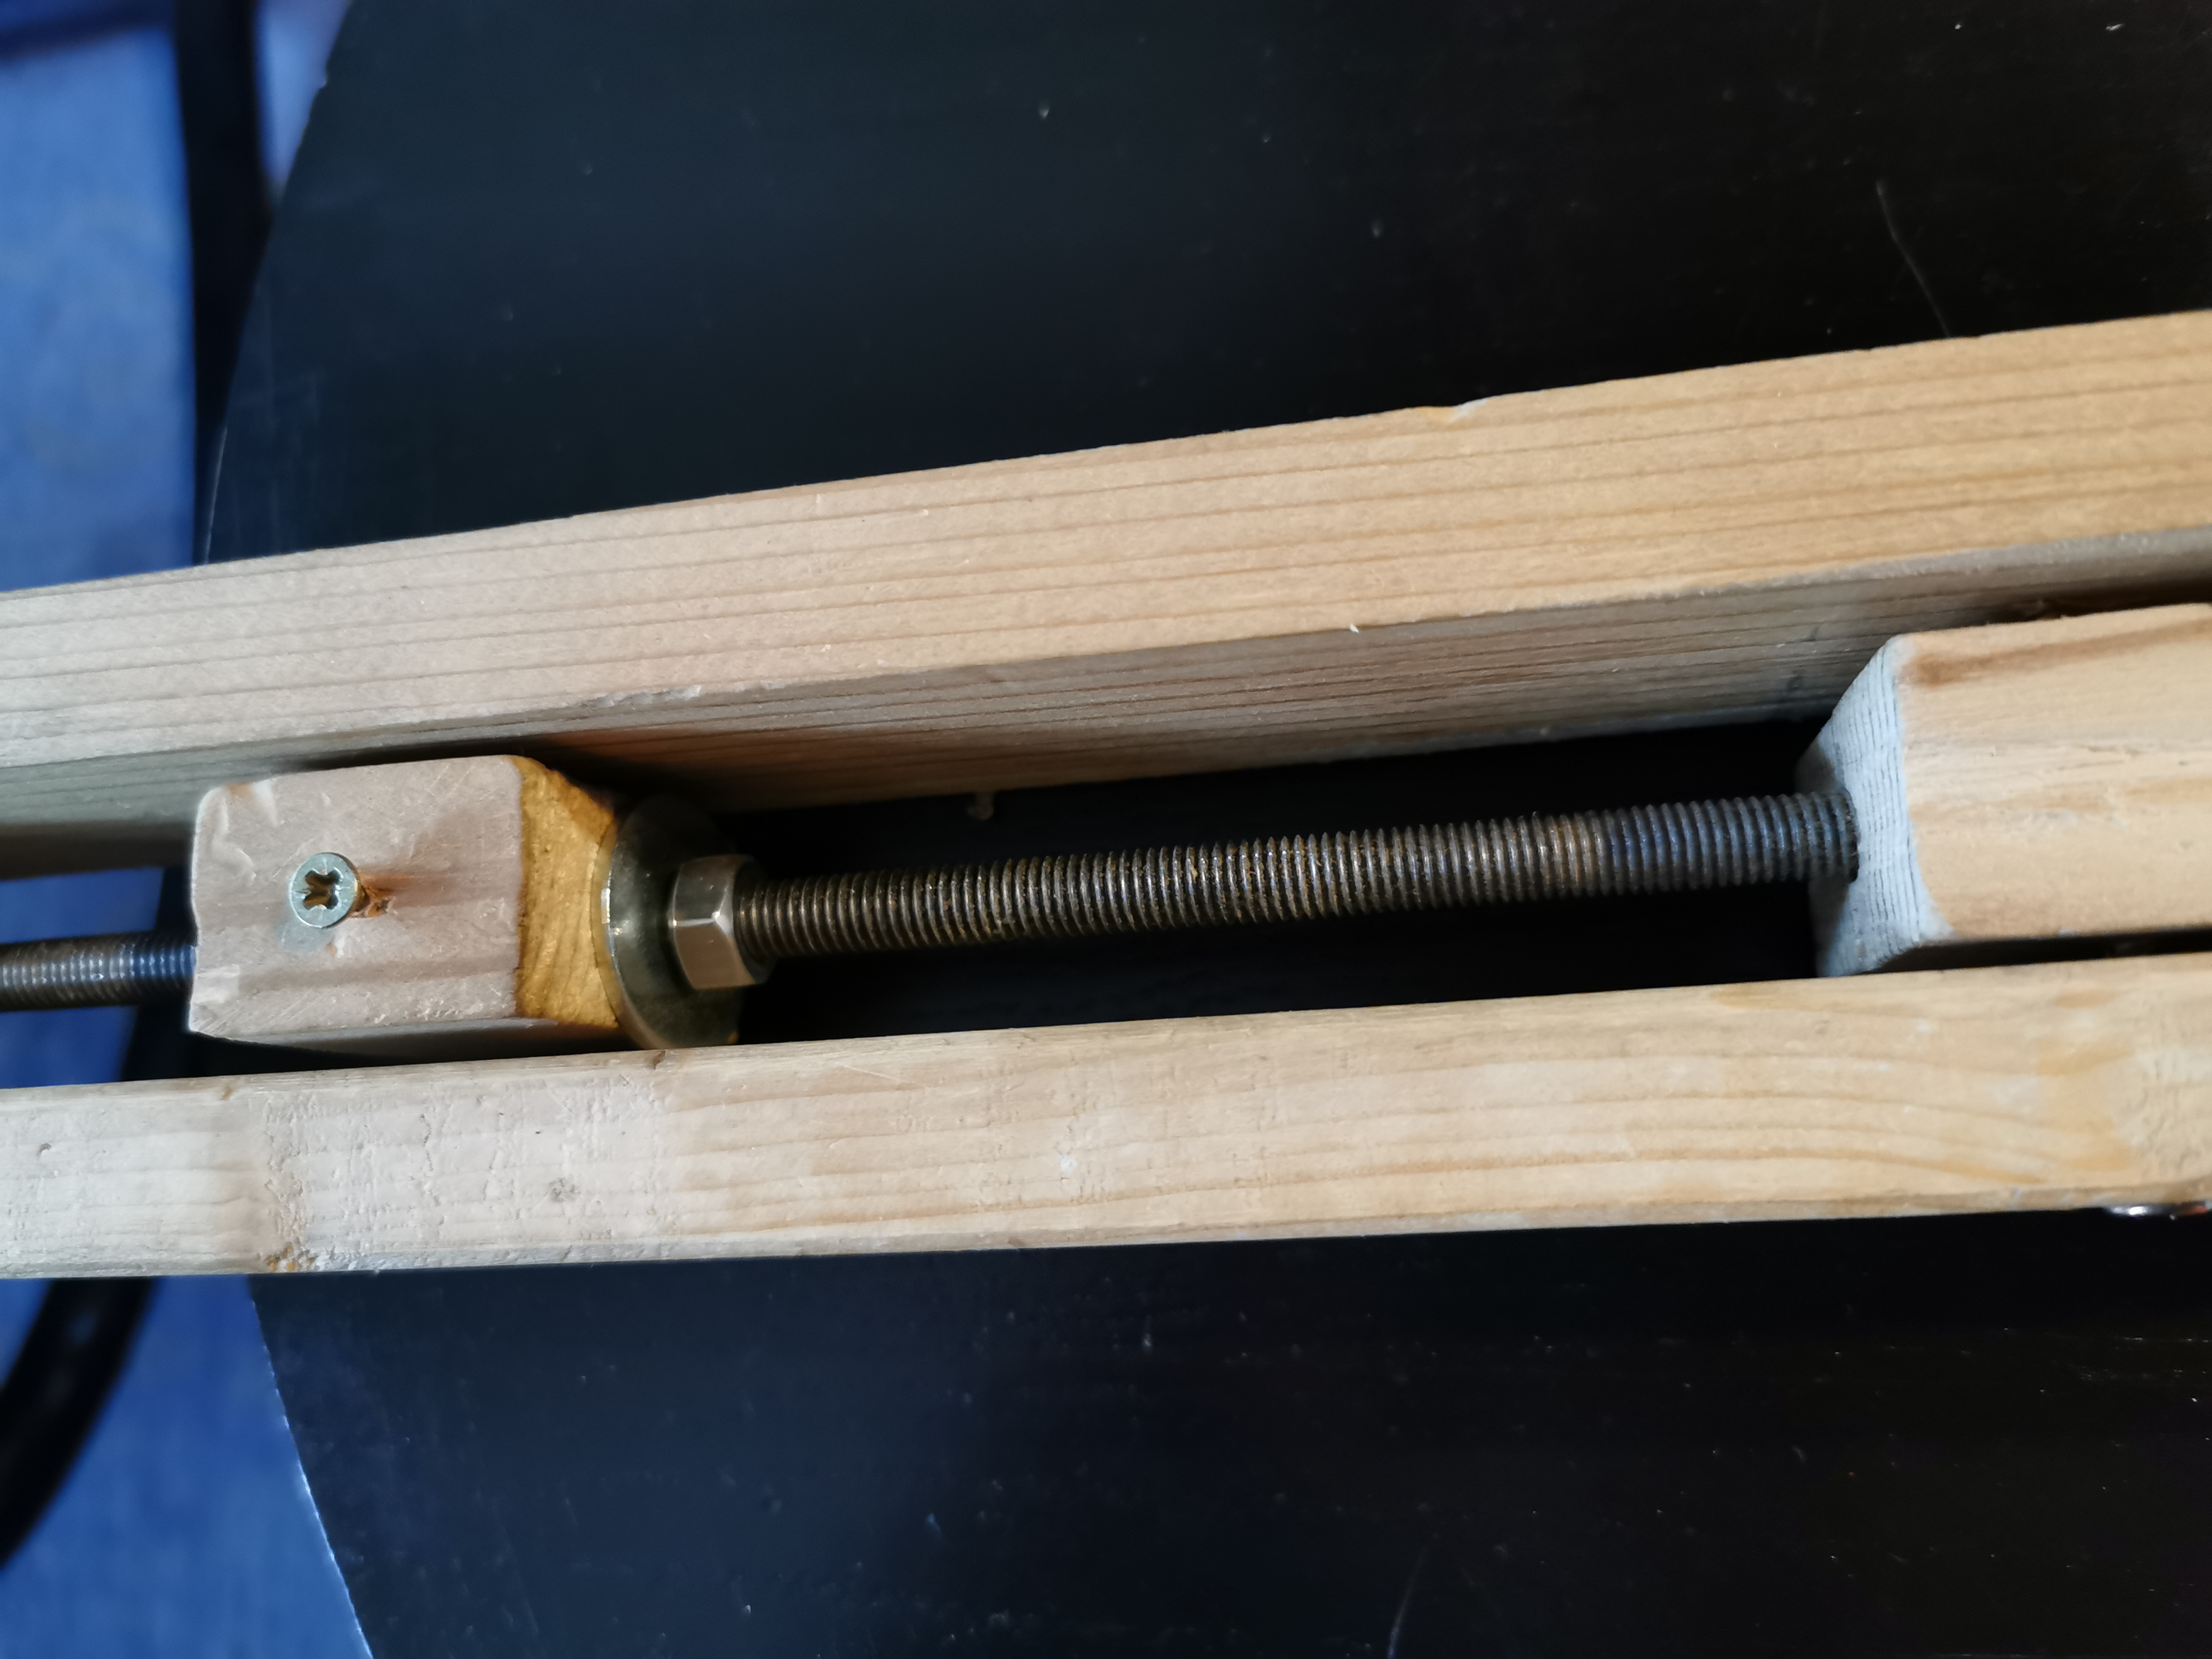
\includegraphics[width=\linewidth]{vegekozel2.jpg}
\end{subfigure}
\caption{}
\label{menetes}
\end{figure}

A méréshez egy A3 és egy E3 hárfahúrt használtuk. Azok hosszát a méréseinknél közepes, $30$\,N feszítőerőnél mértük meg, azokra $L_\text{A} = (72,5 \pm 0,5)$\,cm és $L_\text{E} = (80,5 \pm 0,5)$\,cm adódtak. Sűrűségnek az irodalmi értéket \cite{hur_surusegek}, $\rho = 1150$\,$\kgm$-t használtuk.

% ----------------------------------------------------------------
\subsection{Mérés menete}

A méréshez a két húr alapfrekvenciáit különböző feszítőerők mellett mértük, amit különböző súlyokkal értünk el. Figyeltünk arra, hogy a megfeszítésnél a feszítő kar vízszintes legyen, mert így pontos az erőkar áttétel A mérésnél a Fourier transzformációhoz \emph{Hanning} ablakot használtunk, viszont \emph{Ractangle} ablakkal is hasonló eredményeket kaphatunk. A mért alapfrekvenciákat és a feszítő erőket lejegyeztük.

A mérési eredményeket az \emph{Igor Pro} \cite{igor} szoftverrel értékeltük ki. Ugyanezt \emph{Excellel} \cite{excel} is meg lehet csinálni, viszont ott az illesztésnél nem lehet a mért adatoknak hibát megadni és az illesztésből kapott értékek hibájának kiszámolása is körülményes. Viszont ahhoz, hogy a mérés pontosságáról mondani tudjunk valamit, szükségünk van az eredmény hibájára is.

% ----------------------------------------------------------------
\subsection{Mérési eredmények}

A mérést két húrral is elvégeztük, a mért értékeket a \ref{hur_eredmenyek}.\ táblázatban láthatjuk.

\begin{table}[h!]
\centering
\begin{subtable}[t]{.5\linewidth}
\centering
\begin{tabular}{c | c}

$T$ (N) & $f_0$ (Hz) \\
\hline
 $9,8 \pm 0,5$ & $107,0 \pm 1,5$ \\
$19,6 \pm 1,0$ & $140,0 \pm 1,8$ \\
$29,4 \pm 1,5$ & $161,8 \pm 1,8$ \\
$39,2 \pm 2,0$ & $178,8 \pm 2,4$ \\
$49,0 \pm 2,5$ & $199,0 \pm 2,6$ \\
$58,8 \pm 2,9$ & $213,8 \pm 3,3$ \\
$68,6 \pm 3,4$ & $224,5 \pm 3,0$ \\

\end{tabular}
\caption{A3 húr}
\end{subtable}%
\begin{subtable}[t]{.5\linewidth}
\centering
\begin{tabular}{c | c}

$T$ (N) & $f_0$ (Hz) \\
\hline
 $9,8 \pm 0,5$ & $108,5 \pm 1,2$ \\
$19,6 \pm 1,0$ & $141,8 \pm 1,0$ \\
$29,4 \pm 1,5$ & $169,5 \pm 0,7$ \\
$39,2 \pm 2,0$ & $184,3 \pm 1,0$ \\
$49,0 \pm 2,5$ & $199,8 \pm 1,1$ \\
$58,8 \pm 2,9$ & $211,0 \pm 1,4$ \\

\end{tabular}
\caption{E3 húr}
\end{subtable}
\caption{}
\label{hur_eredmenyek}
\end{table}

Ezeket ábrázolva és a korábbiakban tárgyalt $f(T) = C \sqrt{T + T_0}$ alakú függvényt illesztve rájuk a \ref{f_vs_T}.\ ábrát kapjuk.

\begin{figure}[h!]
\centering
\begin{subfigure}[t]{0.5\linewidth}
\centering
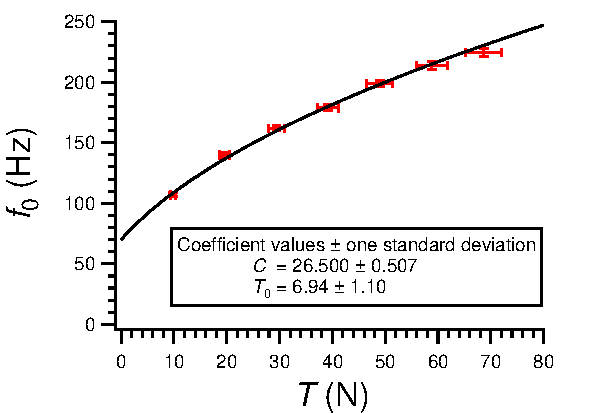
\includegraphics[width = \linewidth]{f_vs_T_A.pdf}
\caption{A3 húr}
\end{subfigure}%
\begin{subfigure}[t]{0.5\linewidth}
\centering
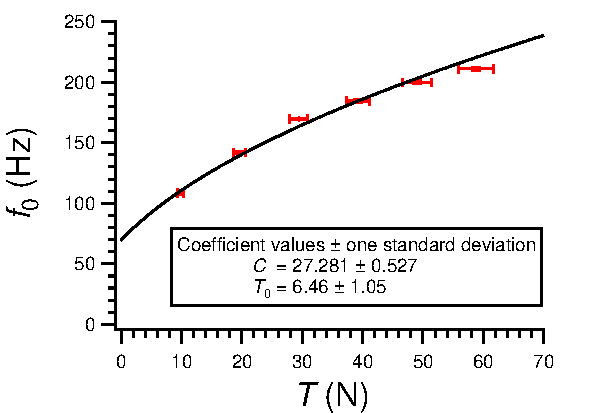
\includegraphics[width = \linewidth]{f_vs_T_E.pdf}
\caption{E3 húr}
\end{subfigure}
\caption{}
\label{f_vs_T}
\end{figure}

Az illesztésekből azt látjuk, hogy $T_0$ értéke mindkét esetben nagyjából ugyanakkora, ami megfelel a várakozásainknak. $C$ értékére pedig $C_\text{A} = (26,500 \pm 0,507)$ és $C_\text{E} = (27,281 \pm 0,527)$ adódnak. Ebből a
$$ d = \frac{1}{C L \sqrt{\rho \pi}} $$
képlet alapján számolhatjuk az átmérőt. A mért $L_\text{A}$ és $L_\text{E}$ értékeket is behelyettesítve $d_\text{A} = (0,866 \pm 0,018)$\,mm és $d_\text{E} = (0,758 \pm 0,015)$\,mm adódnak.

% --------------------------------
\subsubsection*{Méréskiértékelés Excellel}

Ha Excelt szeretnénk az adatok kiértékeléséhez használni, akkor az ábrázolásnál és illesztésnél másképp kell eljárnunk. Itt az A3 húrhoz tartozó mérési eredményeket fogjuk példa képpen kiértékelni.

Mivel az Excelben kevesebb opció van az illesztés paramétereinek megadására és azok rögzítésére, nem tudunk közvetlenül az $f_0$ - $T$ összefüggésre görbét illeszteni. Viszont ha az alapfrekvenciát négyzetre emeljük az
$$ f_0^2 = \frac{1}{d^2 L^2 \rho \pi} T $$
lineáris összefüggést kapjuk. Így az $f_0^2$ - $T$ összefüggést ábrázolva és arra egyenest illesztve megkaphatjuk az átmérőt. Az ábrázolást a \ref{excel_f2_vs_T}.\ ábrán láthatjuk.

\begin{figure}[h!]
\centering
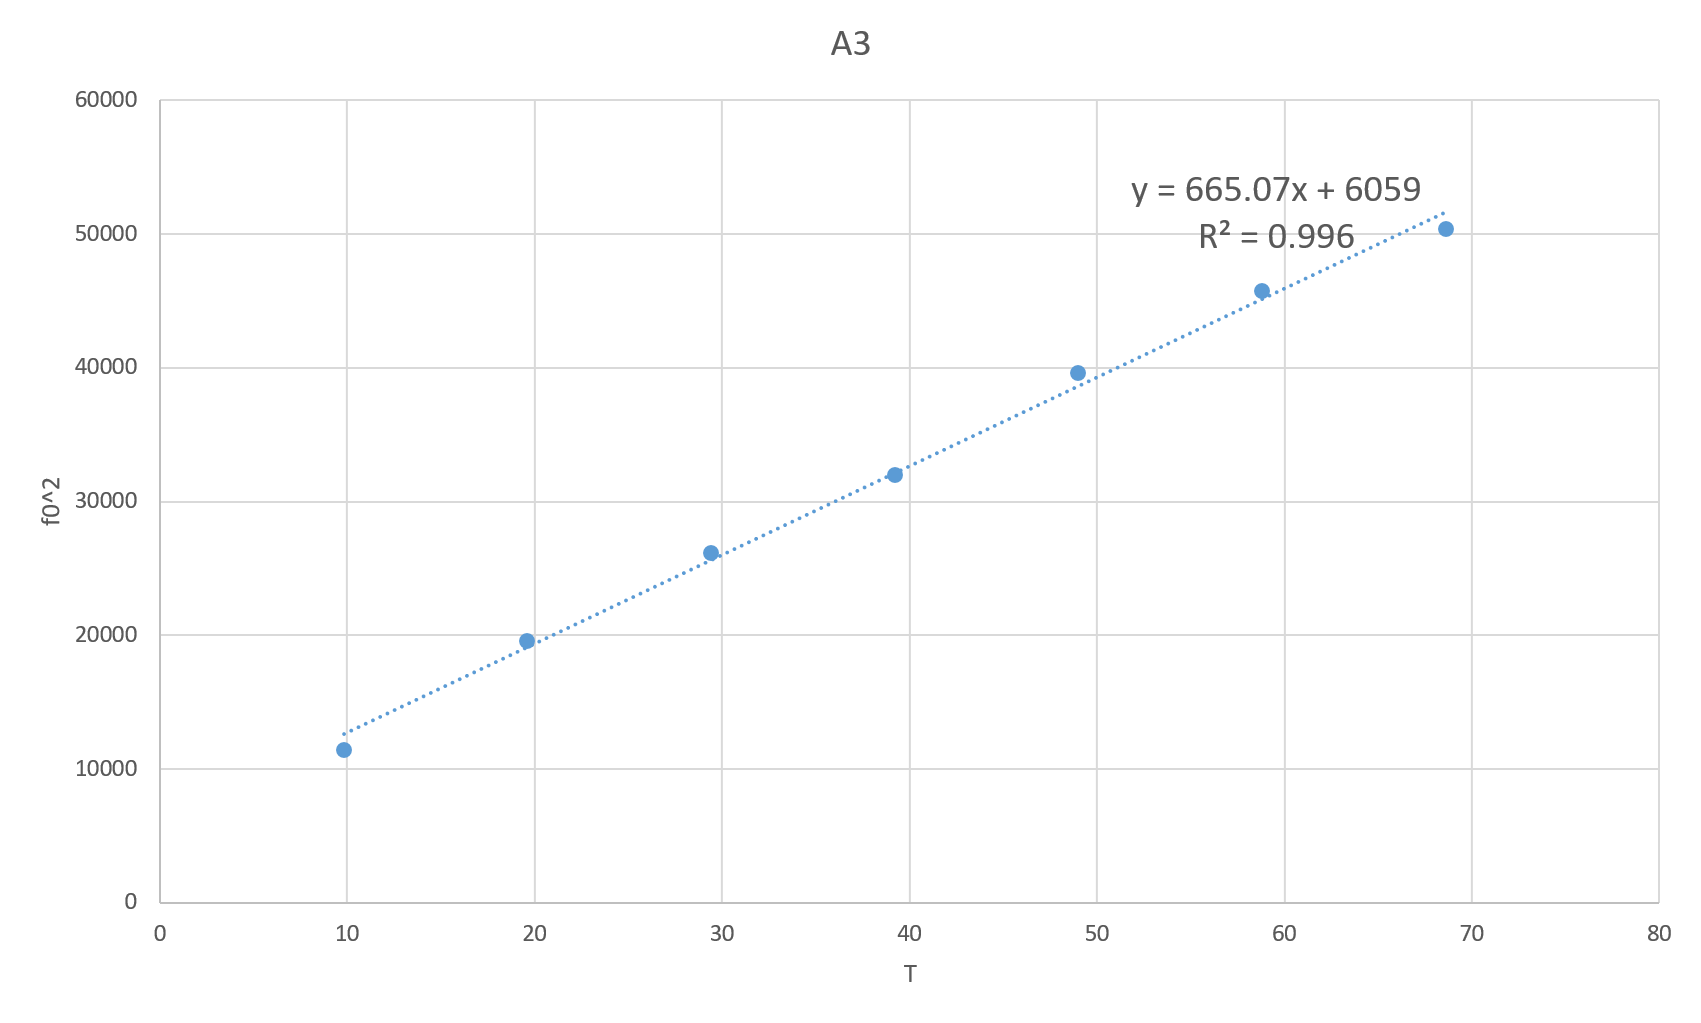
\includegraphics[width = 14cm]{excel_f2_vs_T.png}
\caption{}
\label{excel_f2_vs_T}
\end{figure}

Az illesztésből $C^2 = 665,07$ adódik, így $C = 25,789$. Ezzel az átmérőt kiszámolva $d = 0,890$\,mm adódik. Ez a korábban kiszámolt $d_\text{A}$ értéknek csak kétszeres hibakörnyezetébe esik bele, így azt mondhatjuk, hogy az így számolt érték csupán egy becslés.





% ================================================================

\begin{thebibliography}{h!}

\bibitem{kisfiz1}
Vankó Péter: Kísérleti fizika 1.\ 10.6.\ fejezet \\
\href{http://physics.bme.hu/sites/physics.bme.hu/files/users/BMETE11AF42_kov/KisFiz1.pdf}
{\texttt{http://physics.bme.hu/sites/.../KisFiz1.pdf}}

\bibitem{mintamuszer}
Fizipédia: Állóhullámok megfeszített, rugalmas húrban \\
\href{https://fizipedia.bme.hu/index.php/\%C3\%81ll\%C3\%B3hull\%C3\%A1mok_megfesz\%C3\%ADtett,_rugalmas_h\%C3\%BArban}
{\texttt{https://fizipedia.bme.hu/index.php/ \\Állóhullámok\_megfeszített,\_rugalmas\_húrban}}

\bibitem{hur_surusegek}
\href{https://en.wikipedia.org/wiki/Nylon}
{\texttt{https://en.wikipedia.org/wiki/Nylon}}

\bibitem{igor}
\href{https://www.wavemetrics.com}
{\texttt{https://www.wavemetrics.com}}

\bibitem{excel}
\href{https://products.office.com/en-us/excel}
{\texttt{https://products.office.com/en-us/excel}}

\bibitem{human_voice}
\href{https://en.wikipedia.org/wiki/Human_voice}
{\texttt{https://en.wikipedia.org/wiki/Human\_voice}}

\bibitem{github}
GitHub repository \\
\href{https://github.com/Il-Capitano/myDAQ-2019-2020}
{\texttt{https://github.com/Il-Capitano/myDAQ-2019-2020}}

\end{thebibliography}


\end{document}
